%% LyX 2.2.1 created this file.  For more info, see http://www.lyx.org/.
%% Do not edit unless you really know what you are doing.
\documentclass[english,12pt,openright,twoside,letterpaper]{article}
\usepackage[LGR,T1]{fontenc}
\usepackage[latin9]{inputenc}
\setlength{\parskip}{\medskipamount}
\setlength{\parindent}{0pt}
\usepackage{textcomp}
\usepackage{graphicx}
\usepackage{setspace}
\usepackage[numbers]{natbib}
\usepackage{subscript}
\doublespacing

\makeatletter

%%%%%%%%%%%%%%%%%%%%%%%%%%%%%% LyX specific LaTeX commands.
\newcommand{\noun}[1]{\textsc{#1}}
\DeclareRobustCommand{\greektext}{%
  \fontencoding{LGR}\selectfont\def\encodingdefault{LGR}}
\DeclareRobustCommand{\textgreek}[1]{\leavevmode{\greektext #1}}
\ProvideTextCommand{\~}{LGR}[1]{\char126#1}


%%%%%%%%%%%%%%%%%%%%%%%%%%%%%% User specified LaTeX commands.
% 1in + voffset + topmargin + headheight + headsep + textheight + footskip 
% For PhD thesis we also need an extra inch at the bottom
% 1inch = 72 pt
\setlength{\voffset}{0.0in}
\setlength{\topmargin}{.0in}
\setlength{\headheight}{14pt}
\setlength{\headsep}{22pt}
\setlength{\textheight}{8.5in}
\setlength{\footskip}{40pt}

\makeatother

\usepackage{babel}
\begin{document}

\section*{Literature review}

\addcontentsline{toc}{section}{Literature review and experimental methods}
\setcounter{section}{2}
\setcounter{page}{1}

In this chapter a review of the field of van der Waals' materials
is presented. Graphene's properties and prospects are discussed and
the motivation for van der Waals' heterostructures outlined. Characterisation
of graphene and heterostructures by different methods will be reviewed,
with particular focus on techniques around transmission electron microscopy
(TEM). FIB sample preparation for TEM imaging is reviewed, with particular
attention paid to the challenges of this method when applied to beam
sensitive 2D materials and its limitations. Common image processing
and analysis techniques as applied to cross section images of heterostructures
are discussed in the penultimate section. The final section gives
an overview of density functional theory (DFT) calculations for van
der Waals' heterostructures. DFT was carried out by coauthors of papers
in the following chapters but was not part of the project. Nevertheless,
it is the only technique which provides useful comparison to the quantitative
STEM data presented in subsequent chapters, and so an understanding
of it's merits and shortcomings is useful.

\subsection{Graphene, van der Waals' materials and van der Waals' heterostructures}

It is perhaps a hallmark of success that the name ``graphene'' means
different things to different communities: from a strictly free-standing
single atomic plane of carbon, to a vast field of research encompassing
all atomically thin crystals utilising van der Waals' bonding. For
the purposes of this work, graphene is a two-dimensional (2D) allotrope
of carbon: a single layer of carbon atoms held together by sp\textsuperscript{2}
hybridised bonds to form a hexagonal lattice (see Section \ref{subsec:Graphene_and_vdW_heterostructures}).\citep{novoselov2004electric}
These sheets can be sequentially stacked together to form bilayer,
trilayer e.t.c graphene up to bulk graphite\citep{geim2009graphene},
wherein each graphene sheet is known as a basal plane.\citep{bernal1924thestructure}
Van der Waals' materials can be defined as thick crystals composed
of many layers of graphene or other 2D crystals, such as hexagonal
boron nitride (hBN) and transition metal dichalcogenides (TMDCs).
It should be noted that bulk graphite, and all bulk crystals with
homogenous composition and van der Waals' bonding between atomically
thin sheets, are included in the definition of van der Waals' materials.
An interesting extension of this definition occurs when different
2D crystals are stacked upon one another to form van der Waals' heterostructures.
We address these in the final part of this section. The papers presented
in the following chapters characterise both van der Waals' materials
and van der Waals' heterostructures, and not isolated sheets of 2D
materials.

\subsubsection{Graphene and van der Waals' heterostructures\label{subsec:Graphene_and_vdW_heterostructures}}

In 1947 P R Wallace attempted to explain the electronic properties
of graphite by considering the electronic structure of the individual
graphitic basal planes, finding each ``to be a semi-conductor with
zero activation energy''.\citep{wallace1947theband} This work captured
the essence of the unusual properties a single graphitic sheet would
have, though they proved to be far stranger.

\begin{figure}
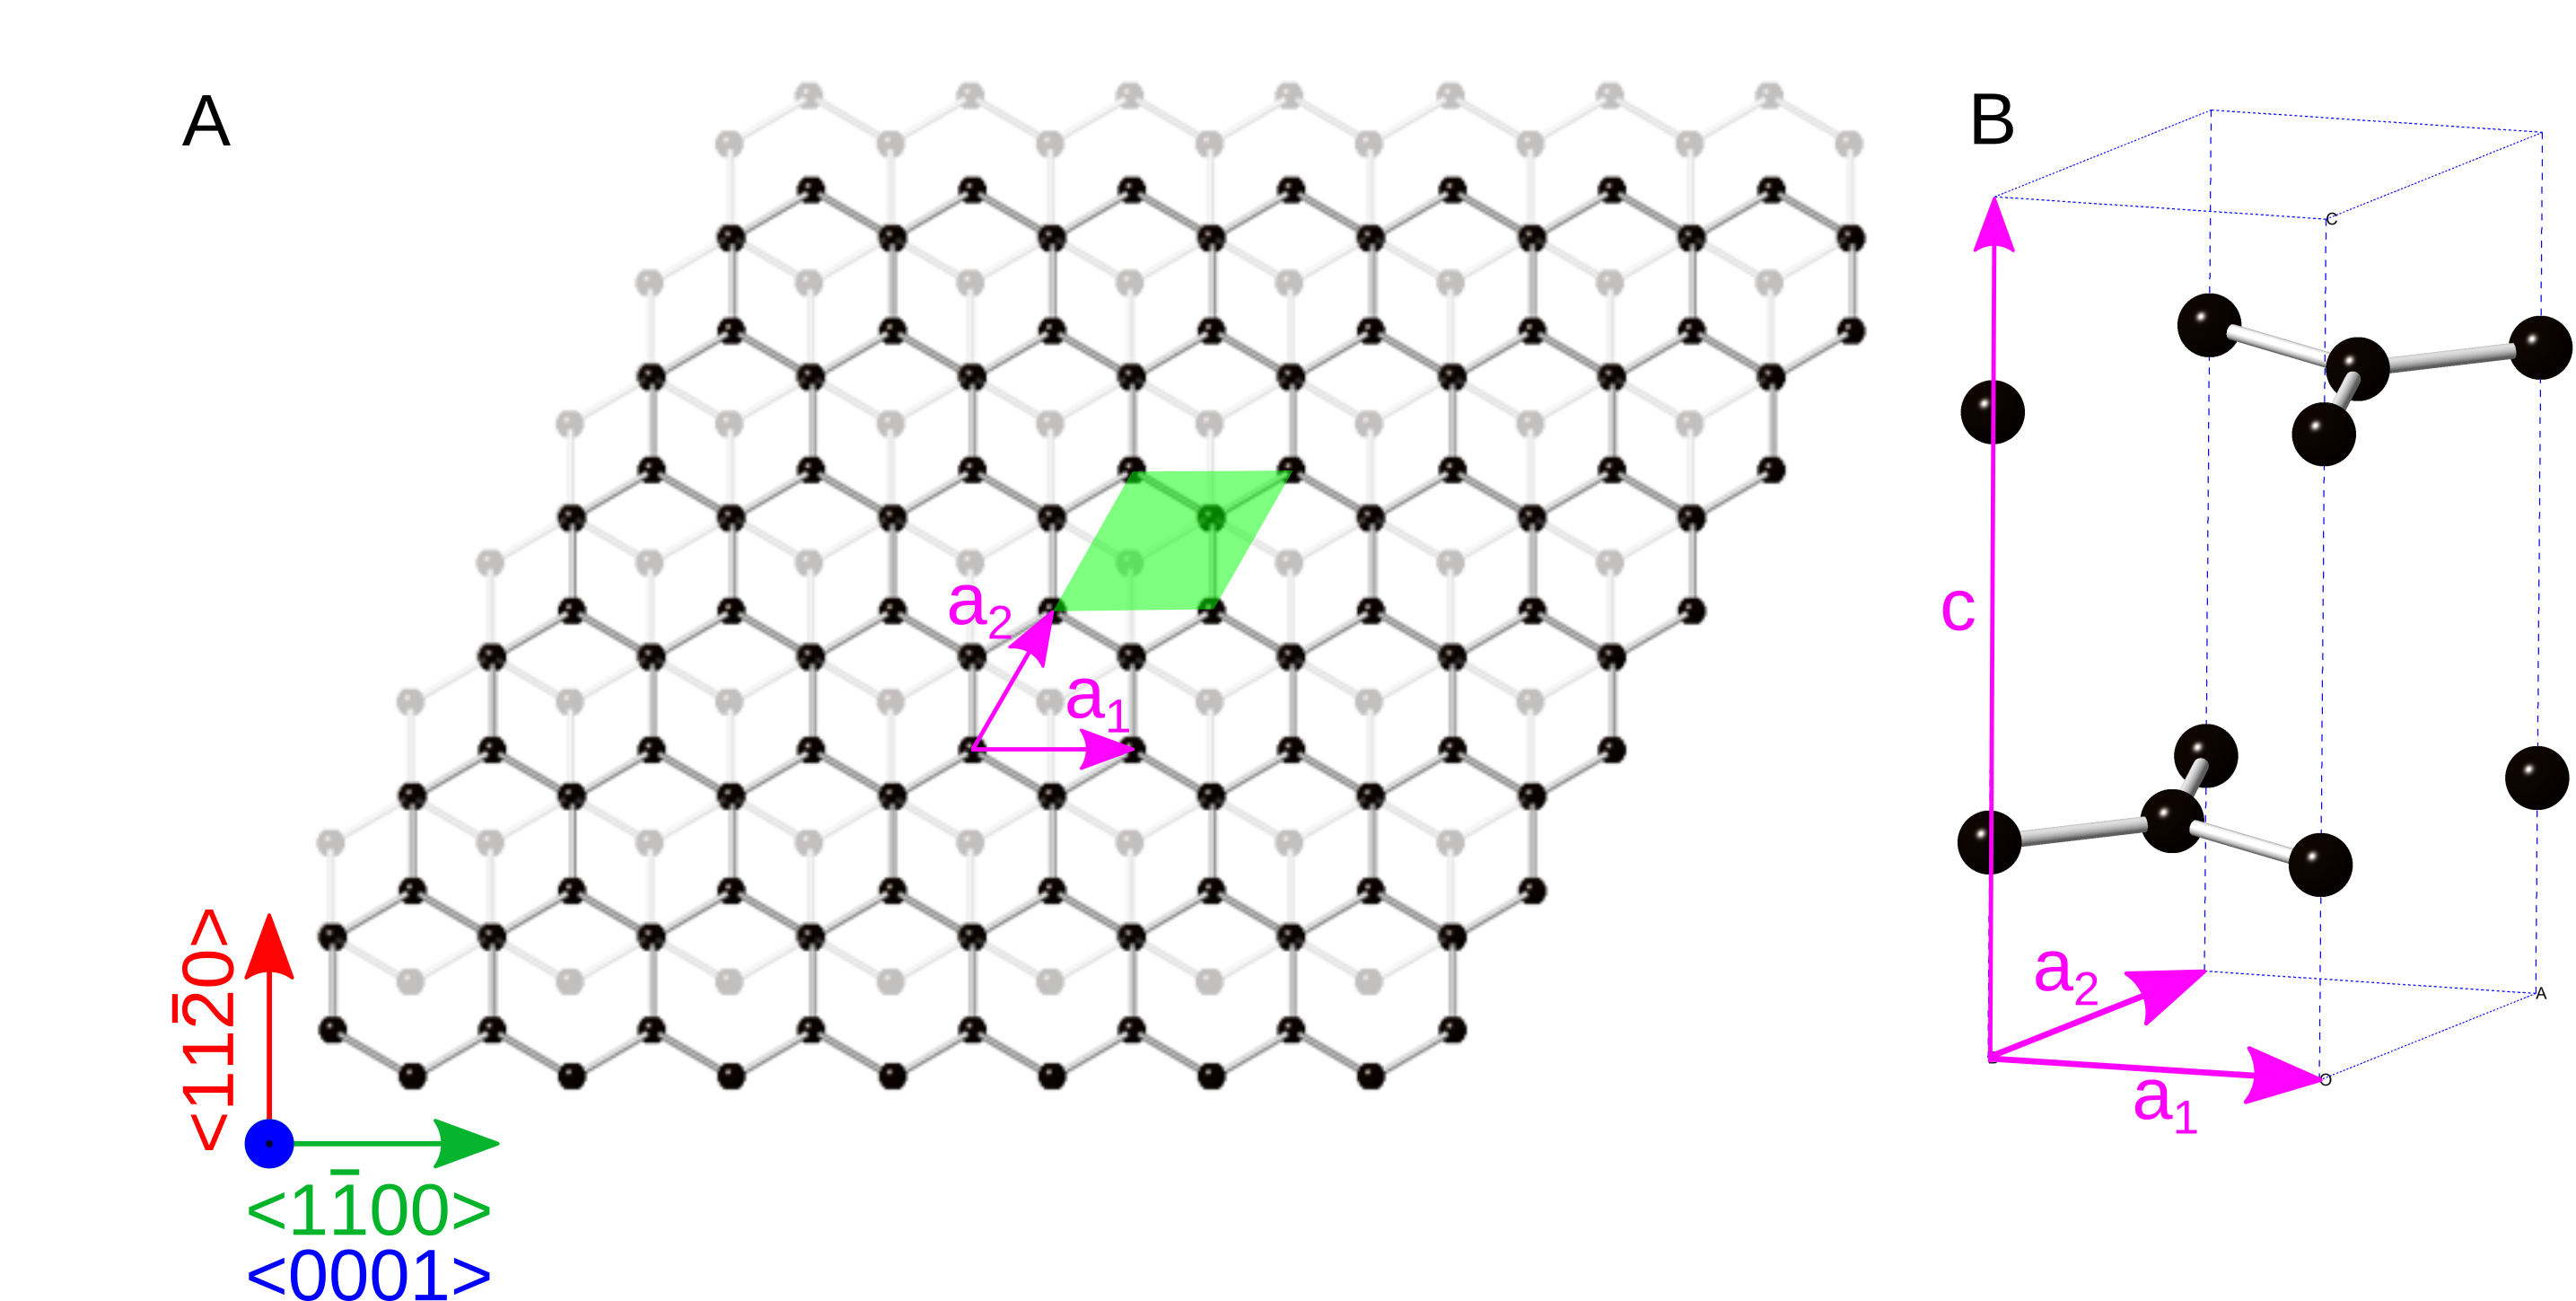
\includegraphics[width=13.5cm]{GraphiteCrystalStructure}

\caption{\textbf{A }Plan view schematic of graphite. The carbon atoms are shown
as black spheres with grey covalent bonds connecting each atom to
three neighbours to form the characteristic 'chicken wire' planar
structure. Two planes can be seen stacked on top of one another, with
the lower plane faded for clarity. Bottom left shows the highest symmetry
crystal directions in graphite. The lattice vectors are drawn in purple
and denoted\emph{ }\textbf{a\protect\textsubscript{1}}\emph{ }and
\textbf{a\protect\textsubscript{2}}, each corresponds to one lattice
translation in the <1-100> or zigzag direction. The planar unit cell
is highlighted green. \textbf{B }Oblique view of the graphite unit
cell highlighted in \textbf{A}, which comprises of two planes of carbon
atoms held together by weak van der Waals' bonding. The lattice vectors
\textbf{a\protect\textsubscript{1}},\emph{ }\textbf{a}\textbf{\emph{\protect\textsubscript{2}}}and
\textbf{c }are drawn.\label{fig:GraphiteCrystal}}
\end{figure}

Graphite is a three-dimensional (3D) allotrope of carbon, and the
most stable form of solid carbon under standard conditions (other
allotropes include diamond, fullerene and carbon nanotubes). It is
the most well known van der Waals material due to its prevalent use
as pencil lead, battery anodes and solid state lubricant. Graphite
has a hexagonal crystal structure with lattice constants of value
\textbf{a }= 2.46 � and \textbf{c} = 6.71 � (see Figure \ref{fig:GraphiteCrystal}B).
The two planes of carbon atoms in the graphite unit cell are entirely
covalently bonded in-plane and the two planes are held together by
van der Waals' bonding. In crystallography these covalently bound
single layers of carbon are labelled as ``basal planes'' when in
graphite, defined as being perpendicular to the principle axis of
the crystal (denoted as \textbf{c}), and the primary plane down which
the crystal can be cleaved. In the growing field of 2D materials,
these planes are thought of as graphene layers stacked on top of one
another. The most favourable stacking configuration in graphite is
that shown in Figure \ref{fig:GraphiteCrystal}, where half of the
carbon atoms sit directly above the neighbouring sites and the other
half sit in the centre of the hexagonal rings to give what is known
as Bernal stacking.\citep{bernal1924thestructure,korhonen2015peeling}
The distance between two basal planes is \textbf{c}/2 = 3.36 �. It
is this large interlayer (basal plane - basal plane) distance, a feature
definitive of these materials which results from the balance of forces
comprising weak van der Waals' bonding\citep{berland2015vander},
which allows atomically thin crystals to be cleaved and isolated from
these materials.\citep{avouris2012graphene}

\begin{figure}
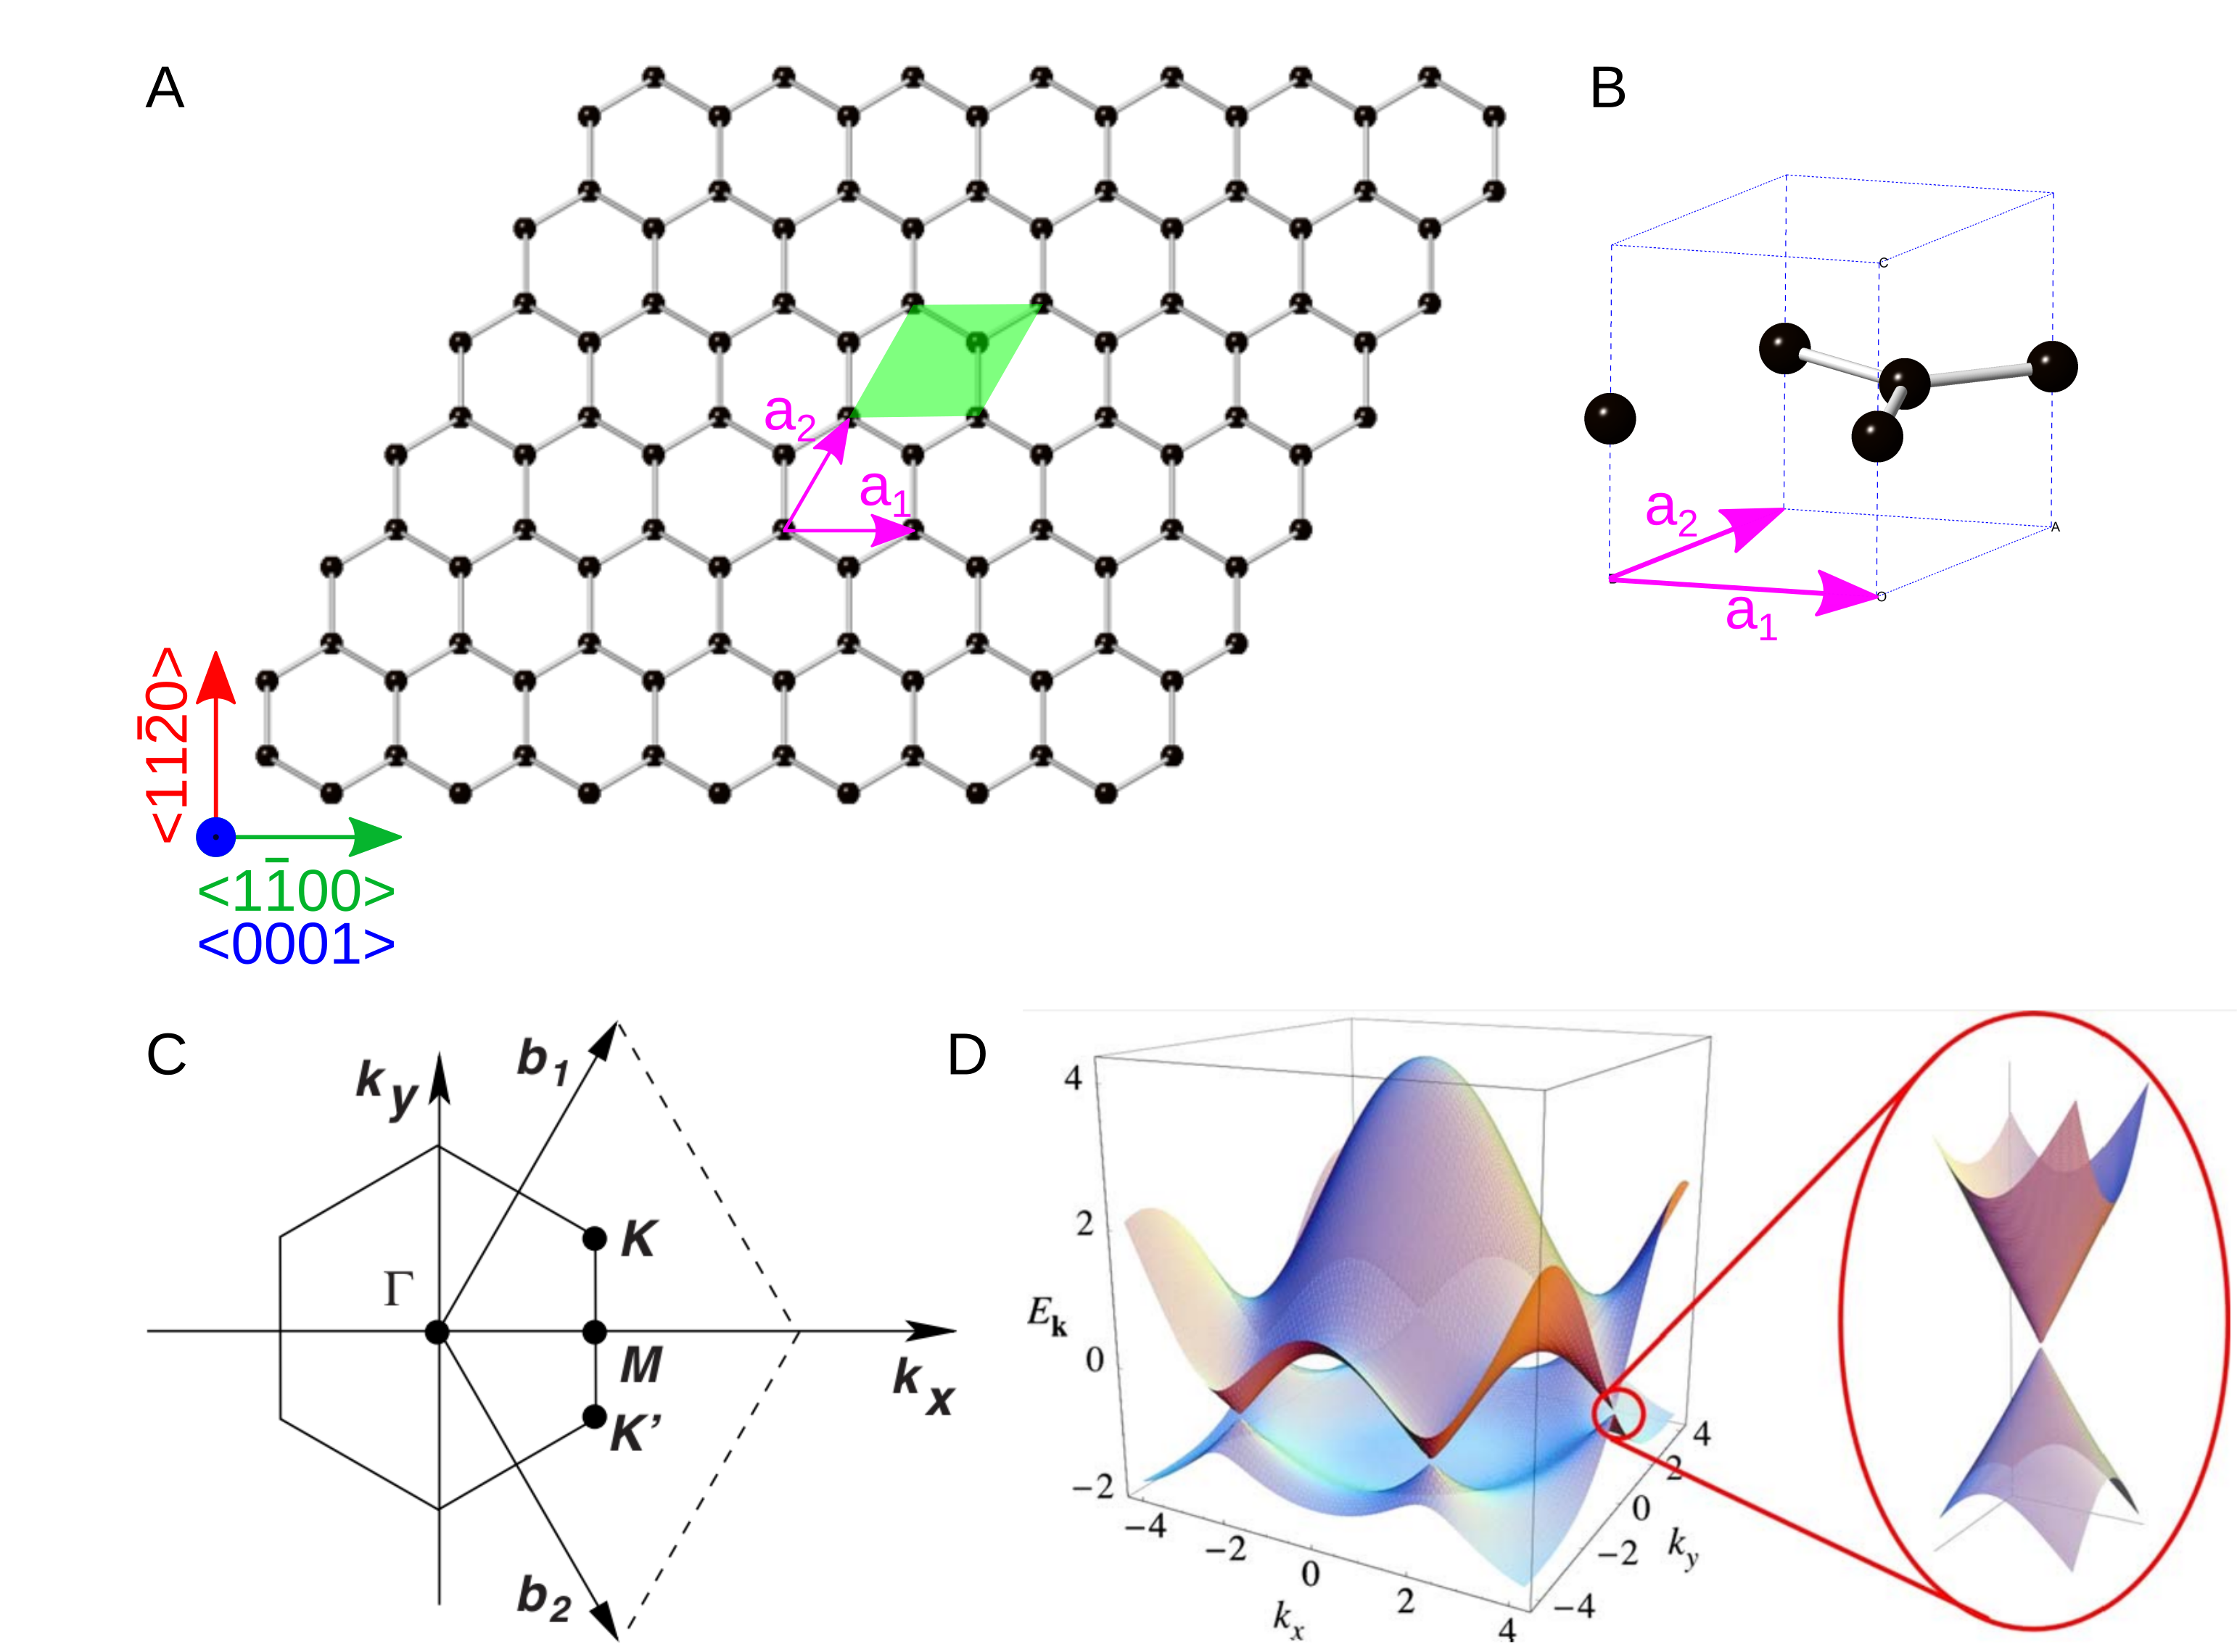
\includegraphics[width=13.5cm]{GrapheneCrystalStructure}

\caption{\textbf{A }Schematic showing an isolated sheet of graphene (a monolayer).
The lattice unit vectors \textbf{a\protect\textsubscript{\textbf{1}}}and
\textbf{a\protect\textsubscript{\textbf{2}}} are drawn as are the
high symmetry directions in the crystal <11-20>, <1-100> and <0001>,
which correspond to the armchair, zigzag and plane-normal directions,
respectively. The unit cell of graphene is highlighted green and contains
two carbon atoms in total. The highlighted unit cell is shown at an
oblique angle in \textbf{B}, where the lattice vectors\textbf{ a\protect\textsubscript{\textbf{1}}}and
\textbf{a\protect\textsubscript{\textbf{2}}} are also drawn.\textbf{
c} is not drawn as isolated graphene is a 2D lattice and does not
require a third lattice vector to describe it (unlike graphite). \textbf{C}
The Brillouin zone of graphene with the reciprocal lattice vectors
\textbf{b\protect\textsubscript{\textbf{1}}}and \textbf{b\protect\textsubscript{\textbf{2}}},
and gamma, M, K and K' high symmetry points are labelled. \textbf{D
}LEFT: The calculated dispersion of electronic states close to the
Fermi level of graphene. RIGHT: The Dirac cones are located at the
K and K\textquoteright{} points with no curvature close to the Dirac
point. Figure reproduced from Castro Neto et al.\citep{castroneto2009theelectronic}
Reprinted (with permission?) from American Physical Society, copyright
2009.\label{fig:GraphENE_crystal_structure}}
\end{figure}

Graphene is an isolated basal plane of graphite, one atom thick and
forming a hexagonal array of carbon atoms connected by strong covalent
bonds (see Figure \ref{fig:GraphENE_crystal_structure}A,B). The valence
electrons of each carbon atom are sp\textsuperscript{2 }hybridised,
allowing an atom to bond to three nearest neighbour atoms and have
electrons left over in an unhybridised 2p\textsubscript{z} orbital
for conduction across the planar lattice. (This can be contrasted
with insulating diamond, where carbon is sp\textsuperscript{3} hybridised
and all valence electrons are engaged in bonding to the four nearest
carbon atoms.) Finally, the two atoms in the unit cell of graphene
belong to two independent sublattices, so that any given atom is bonded
only to those in the opposite sublattice. This has important implications
for charge carriers in graphene. The band structure arising from the
combination of these orbitals and the hexagonal sublattices is unique
and underpins the exotic nature of charge carriers in graphene. Considering
the reciprocal lattice of graphene (shown in Figure \ref{fig:GraphENE_crystal_structure}C)
and using the tight binding approximation, the electronic dispersion
of graphene can be plotted across the Brillioun zone. Where the conduction
and valence bands meet at the K points, there are regions of linear
dispersion which form a zero band gap about the Fermi level. Thus,
graphene is a zero band gap semiconductor or a semimetal. These regions
have been named ``Dirac cones'' and their effect on charge carriers
moving through graphene, and resulting phenomena are explained next.
One final note on the structure of graphene is that a fully relaxed
structure holds static wrinkles which oscillate over tens of nanometre.\citep{meyer2007thestructure}
It is thought that this mechanism stabilises graphene (and other 2D
materials), allowing it to exist as a single sheet of atoms.\citep{fasolino2007intrinsic,geim2007therise}

In 2004 Nobel laureates Prof Andre Geim and Prof Konstantin Novoselov
were the first to successfully isolate and characterise free standing
graphene\citep{novoselov2004electric}, although it should be acknowledged
that monolayer graphite was known prior to this\citep{soule1968directbasalplane,geim2007therise}.
They did this using the 'Scotch tape' method, where micromechanical
cleavage is achieved using sticky tape to pull apart thick highly
oriented pyrolytic graphite until it is atomically thin. The first
electronic transport measurements not only showed that graphene's
band structure has Dirac cones at the K-points of the Brillouin zone,
and that charge carriers close to the centre of the cone behave as
massless Dirac fermions, but that the anomalous quantum Hall effect
and a non-trivial Berry's phase could be experimentally measured in
high quality graphene flakes.\citep{novoselov2005twodimensional,zhang2005experimental}

These phenomena all arise from two fundamental features of graphene's
electronic structure. Firstly, charge carriers in graphene are chiral:
Graphene has two sublattices which both contribute to the wavefunction
of charge carriers, effectively burdoning them with an additional
quantum number ``psuedospin''. Psuedospin sets charge carriers in
graphene apart from other two dimensional electron gases as this additional
property suppresses the backscattering of carriers. Broadly, this
means that exotic quantum mechanical phenomena are more likely to
be observed in graphene than in more traditional condensed matter
systems where scattering can dominate measurements. A surprising manifestation
of this effect is the Klein paradox, where carriers will always propogate
through a sharp barrier if the angle of incidence is 0\textdegree{}
to the barrier normal.\citep{katsnelson2006chiraltunnelling,young2009quantum,wilmart2014akleintunneling}
Graphene also has a unique electronic bandstructure: a gapless, linear
energy spectrum for electrons and holes.\citep{geim2009graphene,castroneto2009theelectronic}
Charge carriers in normal semiconductors can be described by a relatively
straightforward Schr�dinger equation, where the energy and effective
mass varies parabolically. In graphene the Schr�dinger equation is
not applicable to the linear energy spectrum. Instead the charge carriers
must be described by a 2D relativistic Dirac equation as they are
massless about the linear region; thus massless Dirac fermions. This
is the unique case of monolayer graphene. In bilayer graphene an interesting
combination of Dirac and Schr�dinger equations results in massive
Dirac fermions with four possible psuedospin states.

These revelations have propelled graphene to academic and mainstream
fame, with the original Science paper recieving over 21,000 citations,
placing it in the top 100 most cited papers.\citep{vannoorden2014thetop}
Rapid progress in the field revealed monolayer graphene to have carrier
mobilities of up to 200,000 cm\textsuperscript{2 }V\textsuperscript{-1 }s\textsuperscript{-1}at
low temperature in the highest quality devices \citep{chen2008intrinsic,bolotin2008ultrahigh},
but, more interestingly for electronic devices, mobilities upwards
of 15,000 cm\textsuperscript{2 }V\textsuperscript{-1} s\textsuperscript{-1}at
room temperature\citep{geim2007therise}. It was not long before it
was realised that the thin silicon dioxide substrate, which was relied
upon to locate graphene under the optical microscope\citep{blake2007makinggraphene}
and insulate it from the silicon back gate\citep{novoselov2005twodimensional,zhang2005experimental},
was breaking up the 2D electron gas in graphene through surface roughness,
small areas of inhomogenous surface charging and impurities. The device
performance was significantly improved by inserting a thin layer of
insulating hexagonal boron nitride (hBN) between graphene and the
substrate.\citep{dean2010boronnitride}This heralded a step change
in graphene device quality and was one of the first instances of a
van der Waals' heterostructure.\citep{geim2013vander}

\subsubsection{Hexagonal boron nitride: the white graphene}

Monolayer hBN is an insulating isomorph of graphene, sometimes dubbed
``white graphene'', with strong in-plane ionic bonds in place of
graphene's covalent ones.

\begin{figure}
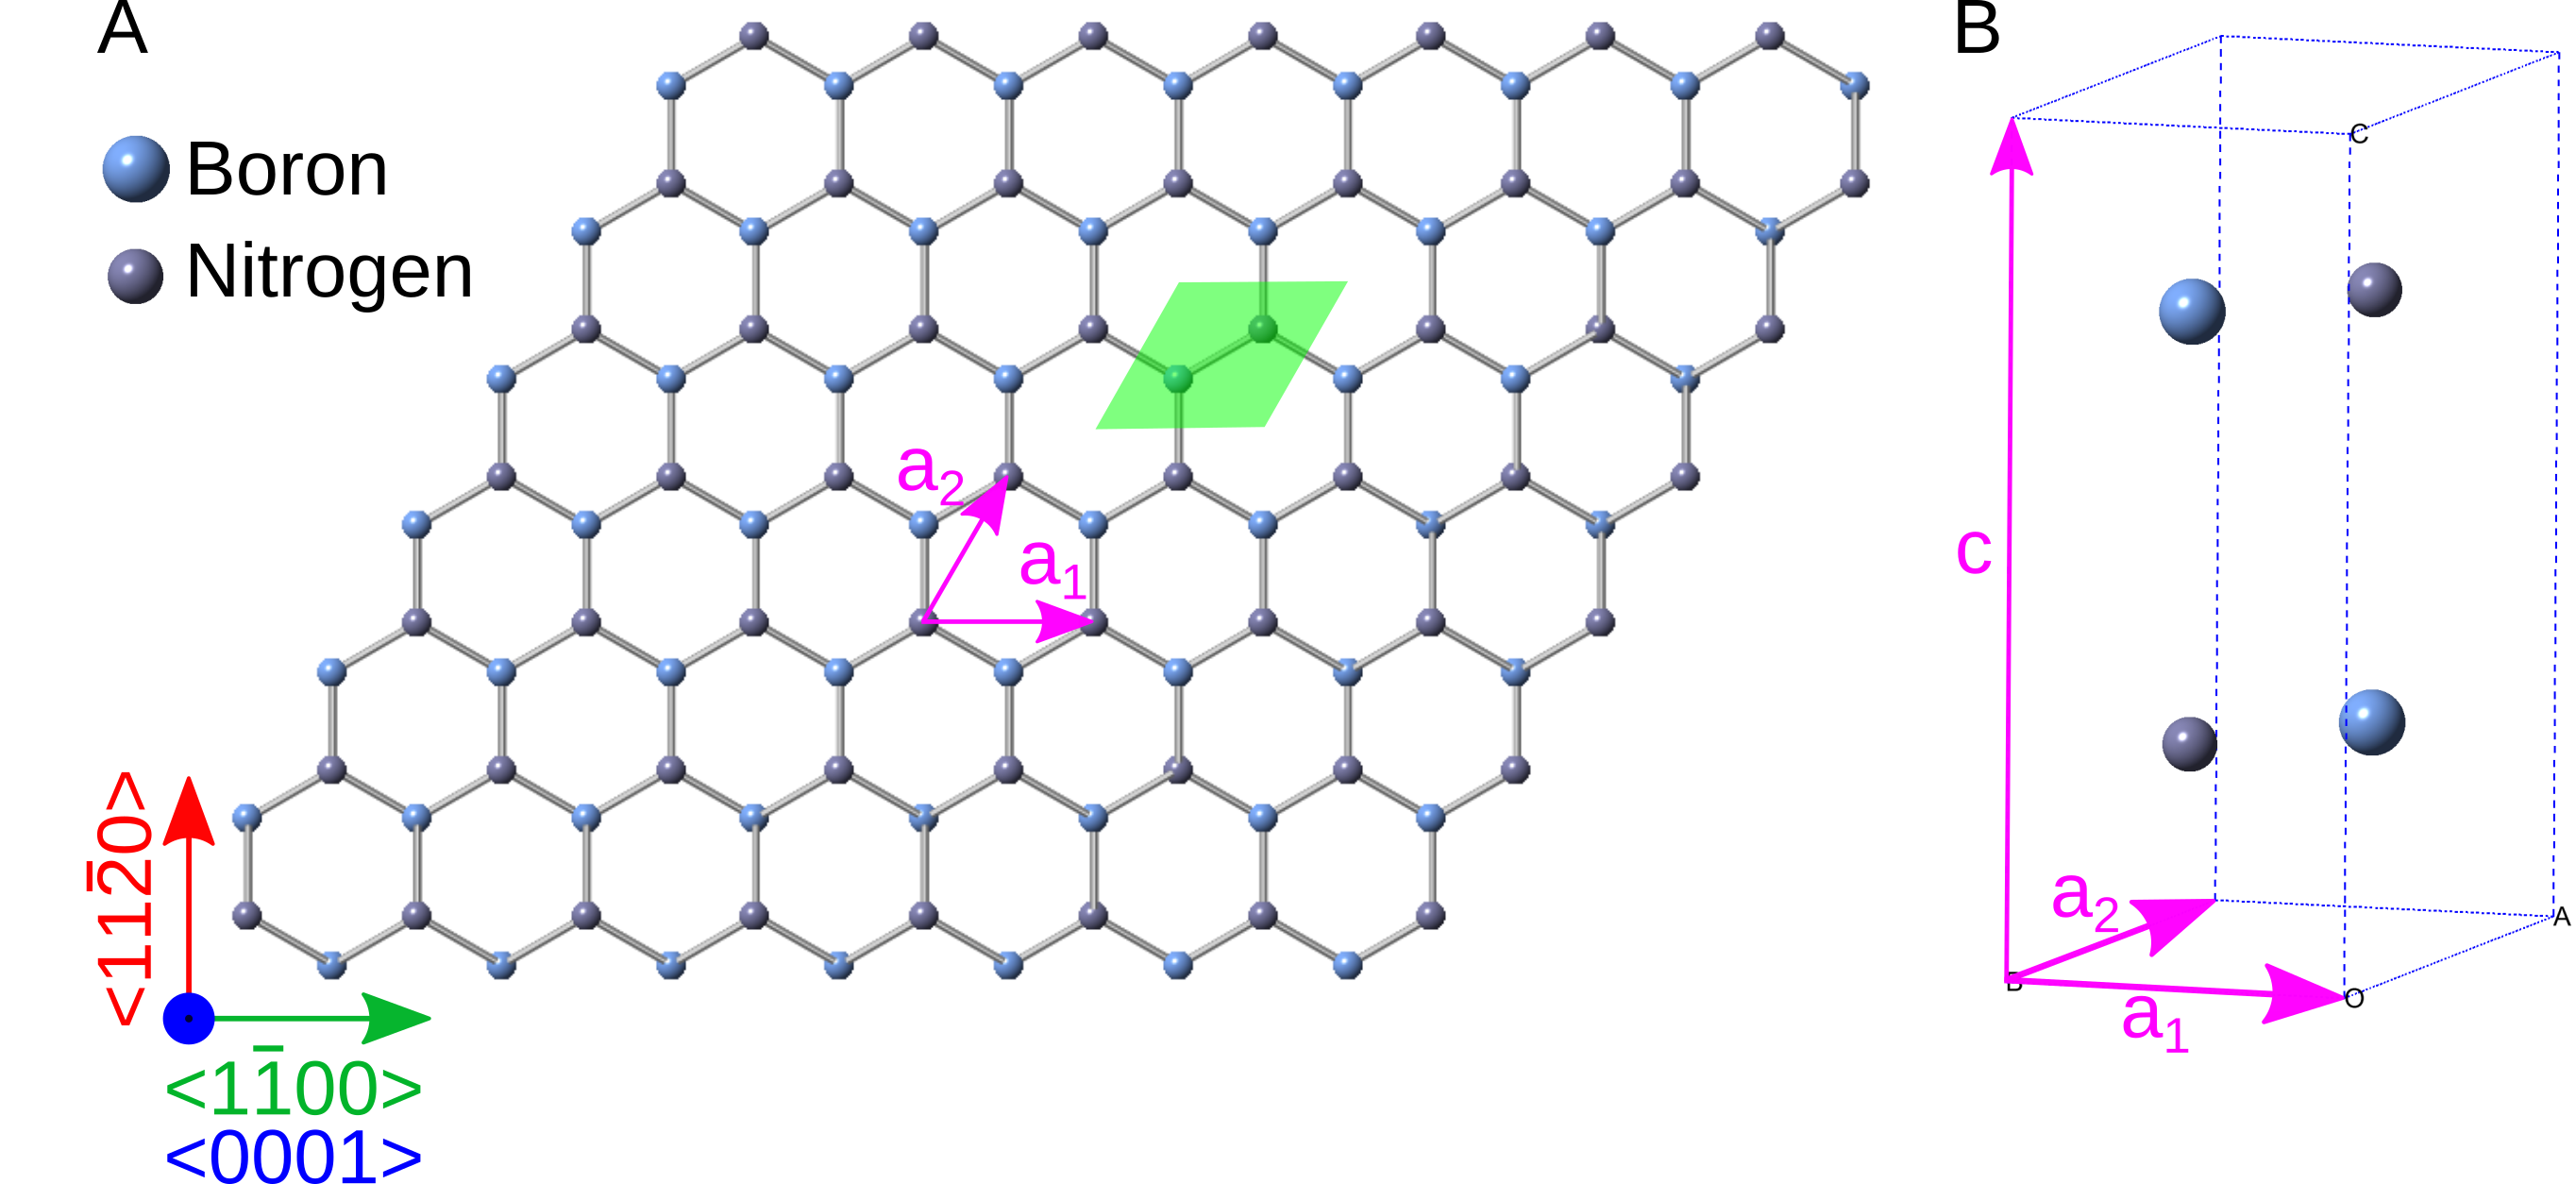
\includegraphics[width=13.5cm]{hBNCrystalStructure}

\caption{\textbf{A} Plan view schematic of hBN structure. Boron atoms are shown
as larger blue spheres and Nitrogen atoms as smaller purple spheres.
The 2D lattice is almost identical to graphene, differing only in
elemental composition and lattice parameters. The lattice unit vectors
\textbf{a\protect\textsubscript{\textbf{1}}}and \textbf{a\protect\textsubscript{\textbf{2}}}
are drawn as are the high symmetry directions in the crystal <11-20>,
<1-100> and <0001>, which correspond to the armchair, zigzag and plane-normal
directions, respectively. The unit cell of hBN is highlighted green
and contains one boron atom and one nitrogen atom. The highlighted
unit cell is shown at an oblique angle in \textbf{B}, where the lattice
vectors\textbf{ a\protect\textsubscript{\textbf{1}}}, \textbf{a\protect\textsubscript{\textbf{2}}}and
\textbf{c} are also drawn.\label{fig:hBN crystal Structure}}

\end{figure}

Bulk hBN glues inert sheets of hexagonal boron and nitrogen lattices
together with van der Waals' bonds, similar to graphite. The lattice
parameters of hBN have values of \textbf{a }= 2.50 � and \textbf{c}
= 6.66 �, which differ only slightly from graphite gives a lateral
lattice mismatch of \textasciitilde{}1.6\%.\citep{woods2014commensurateincommensurate}
hBN prefers AA' stacking, where every boron (nitrogen) atom sits above
a nitrogen (boron) atom of the neighbouring lattice (see Figure \ref{fig:hBN crystal Structure}).\citep{constantinescu2013stacking}
This stacking is highly unfavourable in graphite, which prefers AB
(Bernal) stacking, yet the polar nature of hBN bonding allows the
\textbf{c} lattice parameters for both materials to be nearly identical.\citep{hod2012graphite} 

hBN is a dielectric and , unlike the majority of other 2D materials,
this useful property does not require quantum confinement to be realised.
This means that, as we will discuss later, hBN flakes of different
thickness can be used to separate different conducting components
of a heterostructure and prevent shorting.\citep{britnell2012electron}.
Furthermore, when thin sheets of graphene are placed on top of hBN
and annealed, surface contaminants pool together in bubbles in what
has become known as the self-cleaning phenomenon.\citep{lui2009ultraflat,haigh2012crosssectional,georgiou2013vertical}
Self-cleaning arises from the van der Waals' attraction between hBN
and graphene\citep{khestanova2016graphene} and results in large areas
of atomically clean interfaces, proving vital for high quality measurements.\citep{dean2010boronnitride}
These humble properties have allowed some of the most exciting physical
phenomena to be realised, including negative differential conductance\citep{britnell2013resonant},
Hofstadter\textquoteright s butterfly in bilayer graphene \citep{dean2013hofstadters}
and Klein tunneling of the chiral Dirac fermions.\citep{katsnelson2006chiraltunnelling,young2009quantum,wilmart2014akleintunneling}

\subsubsection{Other van der Waals' materials}

There are an estimated 500 van der Waals' materials which hold the
potential to yield large 2D flakes like graphene.\citep{gibney2015thesuper}
Their properties, and the effects of quantum confinement, are yet
to be predicted for many of them. The 2D crystals that have been isolated
since the discovery of graphene show a diverse spectrum of electronic
properties including metals, semiconductors, insulators and superconductors.
Some of the most recently isolated are silicene\citep{zhao2016riseof},
germanene\citep{davila2014germanene,derivaz2015continuous}, stanene\citep{zhu2015epitaxial},
and phosphorene\citep{liu2014phosphorene} (atomically thin layers
of silicon, germanium, tin and phosphorus, respectively), to name
but a few. Furthermore, some of these 2D materials are expected to
have various structural forms available when atomically thin. For
example, phosphorene is predicted to have two different phases when
monolayer; dubbed blue and black phosphorene, although only the latter
has been realised experimentally.\citep{li2014blackphosphorus,liu2014phosphorene,zhu2014semiconducting,wu2015atomicand}
Many of these materials are unstable under standard conditions and
so research has largely been limited to those that are stable (i.e.
most of the transition metal dichalcogenides and some metal oxides)\citep{geim2013vander},
although specialist handling strategies have being developed for unstable
materials (see Section \ref{subsec:Making-and-transferring graphene})
\citep{cao2015quality}.

One very promising class of 2D materials are the transition metal
dichalcogenides (TMDCs). TMDCs are metallic or semiconducting crystals
of formula MX\textsubscript{2}, where M is a transition metal (e.g.
molybdenum, tungsten, niobium, etc.) and X is a chalcogen (sulfur,
selenium or tellerium). Similarly to graphene and hBN, a TMDC has
sheets of hexagonal crystal structure with strong in-plane bonding.
Each sheet is stacked on top of another and held by van der Waals'
forces. However, unlike graphene and hBN, they are not one atomic
layer but three, with a sheet of transition metal atoms encapsulated
by two sheets of chalcogen atoms. The most popular TMDCs are currently
MoS\textsubscript{2}, WS\textsubscript{2}, MoSe\textsubscript{2}and
WSe\textsubscript{2} due to them having an indirect semiconducting
band gap in bulk crystals and a direct gap in monolayer crystals.\citep{mak2010atomically,splendiani2010emerging,zhang2014directobservation}
The direct band gaps of the popular semiconducting TMDCs range from
roughly 1.5 - 2.1 eV\citep{wang2012electronics}, which correspond
to near infrared - yellow photon energies in the visible spectrum.
Furthermore, these monolayers are ``multivalley semiconductors'',
meaning they have favourable and distinct localised states which a
charge carrier wavefunction can occupy. These states appear as valleys
at the K points of the Brillouin zone (K and -K in Figure \ref{fig:Liu_introTMDCstruc}),
with differences between valleys arising from a lack of inversion
symmetry in the crystal structure of monolayer TMDCs. A carrier can
be confined to one of these valleys and so gains an extra constraint:
a \emph{k}-valley index (also known as valley degree of freedom or
valley pseudospin). In addition to this, semiconducting TMDCs show
strong spin-orbit coupling which arises from the valence electron
states originating from d-orbitals. This results in spin up and spin
down carriers having different energies as spin degeneracy is removed
from the conduction and valence bands.

\begin{figure}
\includegraphics[width=13.5cm]{\string"Liu TMDCs PhysRevB 2013\string".png}

\caption{\textbf{a }Plan view schematic of a monolayer TMDC with chalcogen
atoms shown as small yellow spheres and transition metal atoms shown
as large grey spheres. The 2D unit cell is highlighted green and has
lattice constant \emph{a}. \textbf{\emph{R\protect\textsubscript{1}}}
to \textbf{\emph{R\protect\textsubscript{6}}} shows the nearest neighbour
tranition metal atoms to the centre transition metal atom.\textbf{\emph{\noun{
}}}\textbf{b }Oblique view of a metal atom with trigonal prismatic
coordination to six nearest neighbour chalcogen atoms. The location
of such a site is denoted by the blue triangle in \noun{a. }\textbf{c
}The Brillouin zone with basis vectors \textbf{\emph{b\protect\textsubscript{\emph{1}}}}\emph{
}and \textbf{\emph{b}}\textbf{\protect\textsubscript{\emph{2}}}.
The two valleys \emph{K }and \emph{K-} are shown. {[}build your own
figure..{]} \label{fig:Liu_introTMDCstruc}}
\end{figure}

These phenomena manifest themselves in the form of optical selection
rules in semiconducting TMDC monolayers (although not present in bilayers
or thicker). As with normal semiconductors, charge carriers can be
promoted from the valence band to the conduction band. However, the
spin states in each band are different for the K and -K valleys and
can be selectively excited using left- and right-handed circularly
polarised light.\citep{cao2012valleyselective,kioseoglou2016optical}
This selectivity arises from angular momentum conservation and time
reversal symmetry constraints.\citep{xu2014spinand}

Another attractive feature of semiconducting TMDCs is their exotic
exciton physics. Promotion of carriers in monolayer semiconducting
TMDCs cause electron hole pairs to form strongly bound exciton states
due to the enhanced Coulomb interaction between the carriers that
results from 2D confinement.\citep{klots2014probing,poellmann2015resonant}
These unique properties of semiconducting TMDCs allow a plethora of
physical phenomena to be explored\citep{xiao2012coupled,mak2014thevalley,newaz2013electrical}
and ultimately find application in ultrasensitive photodetectors\citep{lopez-sanchez2013ultrasensitive,tsai2013fewlayer}
and energy harvesting applications\citep{bernardi2013extraordinary}.

The second class of 2D TMDCs are metallic: niobium diselenide, niobium
disulfide, tantallum diselenide and tantallum disulfide, although
their band structure can potentially be made semiconducting if formed
into nanoribbons.\citep{li2013metalto} Niobium diselenide is of particular
interest currently as, if cooled sufficiently, charge density waves
are observed.\citep{wilson1975chargedensity} These take the form
of an ordered fluid of electrons that flow in a highly correlated
but 'bumpy' manner through a material, and is thought to be linked
to an unconventional form of superconductivity in layered materials.\citep{xi2015strongly}
Their occurance in 2D materials has not been fully explained theoretically
and so they are of great interest to fundamental research in condensed
matter physics.\citep{chatterjee2015emergence,ugeda2016characterization}

Bilayer (and thicker) TMDCs are capable of forming different stable
structural polytypes (stacking orders) which often lead to modification
of the electronic properties.\citep{voiry2015phaseengineering} Furthermore,
within these polytypes different polymorphs of the monolayers are
possible i.e. where the metal atom is trigonally or octahedrally coordinated.
Isolated monolayer TMDCs can have different polymorphs (metal atom
coordination) but not polytypes as they are not stacked. In thicker
TMDCs the most common polytypes are 1T, 2H and 3R, where each letter
stands for trigonal, hexagonal and rhombohedral, respectively. The
digits denote the number of monolayers in the unit cell. The dominant
phase in a TMDC crystal is largely down to how the crystal was synthesised
and its disposition towards a polymorph.\citep{shmeliov2014unusual,voiry2015phaseengineering}
For example, MoS\textsubscript{2} is most stable in the 2H phase
with the metal atom trigonally coordinated, whereas TiS\textsubscript{2 }takes
the 1T phase where the metal is octohedrally coordinated. Multiple
phases can even coexist within a flake and can arise during synthesis\citep{enyashin2013linedefects,lee2016ramansignatures}
or patterned using electron beam irradiation\citep{lin2014atomicmechanism}.
Finally, azimuthal rotation of monolayers relative to one another
creates variations in stacking via a moir� effect but does not seem
to yield distinct and different polytypes \citep{puretzky2016twisted}. 

\subsubsection{Potential applications of graphene}

In addition to graphene's incredible electronic merits are a host
of other properties which are unrivalled by other materials. It is
the thinnest imaginable material (one atom thick)\citep{novoselov2004electric};
nearly completely optically tranparent\citep{nair2008finestructure},
has the largest specific surface area (2630 m\textsuperscript{2}
g\textsuperscript{-1})\citep{bonaccorso2015graphene}; the strongest
and stiffest material ever measured (Young's modulus of 1 TPa and
intrinsic strength of 130 GPa)\citep{lee2008measurement}; has the
highest thermal conductivity (> 3,000 W mK\textsuperscript{-1})\citep{balandin2011thermal};
the highest tolerance of electronic current density (a million times
that of copper)\citep{moser2007currentinduced,murali2009breakdown}
and longest mean free path of electrons under ambient conditions\citep{tse2008ballistic};
the most stretchable crystal\citep{guinea2010energygaps} and is impermiable
to gases\citep{bunch2008impermeable}. 

These myriad superior properties (most of which are only observed
in the highest quality flakes) make graphene an ideal candidate for
many applications.\citep{novoselov2012aroadmap,ferrari2015science}
Graphene-based inks and paints are expected to provide conductive
inks, antistatic and interference shielding, corrosion barriers and
gas membranes.\citep{kirkland2012exploring,yoo2014graphene,su2014impermeable,wang2015electrical,cui2016gasbarrier}
Transparent conductive coatings for consumer flexible electronics
(e.g. flexible touch screens and rollable electronic paper) are already
being researched commercially.\citep{bae2010rolltoroll,ahn2014graphene,samsung}
By embedding graphene in polymer or ceramic matrices a new class of
superstrong, lightweight and degradation resistant composites are
anticipated to emerge over the next ten years.\citep{kim2010graphenepolymer,verdejo2011graphene,young2012themechanics}
Graphene based composites are also poised to play important roles
in boosting the performance of many electrochemical and optoelectronic
applications such as energy harvesting and storage technologies (fuel
cells, supercapacitors, batteries, etc.).\citep{huang2012graphenebased}
The properties of graphene are extremely sensitive to environment
and can be used in many different sensor applications. These range
from drilling holes in graphene in order to sequence DNA\citep{feng2015identification,paulechka2016nucleobasefunctionalized},
to flakes acting as intrinsic strain gauges via Raman spectroscopy
characterisation\citep{neumann2015ramanspectroscopy,delcorro2015strainassessment}.
Other sensing applications include gas environment, pressure and magnetic
field, with devices possibly measuring many of these metrics simultaneously.\citep{chen2012optical,zhao2013infrared,huang2015multifunctional,schedin2007detection}
Graphene is easily functionalised\citep{kuila2012chemical,georgakilas2016noncovalent}
yet relatively inert which opens up possibilities in bioapplications,
particularly in biomolecular sensing, tissue engineering, regenerative
medicine and drug delivery.\citep{hirtz2013multiplexed,liu2013graphene,goenka2014graphenebased}

It is widely anticipated that graphene will make it's biggest impact
in the fields of electronics and photonics.\citep{castroneto2009theelectronic,avouris2010graphene,schwierz2010graphene,bao2012graphene,bonaccorso2010graphene}
The poignant absence of a band gap in monolayer and bilayer graphene
all but eliminates it's application as a speedy and direct replacement
for silicon in conventional logic gate archetectures. Nevertheless,
there are currently three stratagies to open a band gap in graphene:
confining the width of graphene to form nanoribbons\citep{chen2007graphene,li2008chemically},
biasing bilayer graphene\citep{castro2007biasedbilayer,ohta2006controlling,zhang2009directobservation},
and straining graphene\citep{pereira2009tightbinding,ni2008uniaxial}.
Monolayer graphene nanoribbons currently show the most promise with
bandgaps scaling inversely with the width of the ribbon, in some cases
reaching 200 meV for < 20 nm widths\citep{chen2007graphene,li2008chemically}.
However, amongst problems relating to reproducible ribbon quality,
confined carriers rapidly lose mobility and risk negating any advantages
over silicon. The main motivation for integrating graphene in logic
devices is to extend the trend in integrated circuit advancement as
professed by Moore's Law, which in turn forms the basis of financial
growth for the semiconductor industry.\citep{moore2003noexponential,schwierz2010nanometer}
Through reduction in the size of silicon metal-oxide-semiconductor
field-effect transitors (MOSFETs) the performance of integrated circuits
has roughly doubled every 18 months for the last fifty years.\citep{schwierz2010graphene}
However size reduction is rapidly approaching it's limit in silicon
and new materials are being sought to increase device performance
and decrease feature size.\citep{itrsnews} Although mobility is typically
cited as graphene's most attractive feature for high speed logic devices,
it is actually the potential to have robust single atom channel widths
which sustains interest within the semiconductor community (despite
a lack of bandgap).\citep{schwierz2010graphene} New device concepts
are being explored to work around graphene's shortcomings, the most
promising of which is the bilayer pseudospin FET; two graphene monolayers
separated by a similarly thin dielectric. To switch the device on
a gate bias is applied which encourages carriers to tunnel through
the dielectric, effectively creating a short circuit current to flow
through the channel. Under different bias conditions the tunnelling
resistance is high, suppressing tunnelling and switching the device
off.\citep{banerjee2009bilayer} This is anticipated to yield high
on-off ratios with a very low switching energy.

The unique optical properties of graphene make it an excellent candidate
material for many photonic devices. Photodetectors, mode-locked lasers,
polarizers, isolater devices and optical modulators are all anticipated
applications for graphene's optical properties, many of which already
have proof of concept devices.\citep{eberlein2008plasmon,ju2011graphene,kim2011graphenebased,chen2012optical,fei2012gatetuning,grigorenko2012graphene,polat2013broadband,wang2013highresponsivity,yan2013damping,marshall2013electronically,chakraborty2016gainmodulation}
Optical modulators are key components in photonics systems as they
are used to control the characteristics of light packets carrying
signals between devices.\citep{luo2015graphenebased} Modulation speed,
the spectral range of the modulator, energy consumption and device
size all dictate the quality of an optical modulator, and all of which
depend on modulating material. Graphene is particularly useful for
optical modulation for three reason: Graphene has a high modulation
speed owing to it's intrinsically high carrier mobility; the absorption
and modulation characteristics can be directly controlled by changing
the Fermi level using a gate bias; and graphene has a large optical
bandwidth with a constant absorption of 2.293\% from the infrared
to visible wavelengths (which happens to coincide with the optical
communication bandwidth required).\citep{luo2015graphenebased2,polat2013broadband}
This absorption may seem low, however when taken into consideration
with graphene's single atom thickness it is in fact very high compared
to other photonics materials. These properties could prove most lucrative
in terahertz modulators and detectors, which would begin to bridge
what has become known as the ``terahertz gap'' and pave the way
to cheap and powerful long wavelength applications.\citep{ju2011graphene,rahm2012thzwave,marshall2013electronically}

The main bottlenecks to progress in all these areas lie in the fundamental
problems of handling graphene and scaleable synthesis.

\subsubsection{Making and transferring graphene flakes\label{subsec:Making-and-transferring graphene}}

The papers presented in the following sections of this thesis use
devices made from mechanically exfoliated 2D flakes. For context a
brief review of other synthesis routes to graphene flakes are presented
here.

The myriad different methods for synthesising graphene flakes fall
broadly under mechanical exfoliation, chemical growth and liquid phase
exfoliation. Exfoliation methods are considered ``top-down'' synthesis
routes as they directly remove graphene sheets from a bulk crystal
of graphite. Chemical growth methods are ``bottom-up'' as they typically
use a carbon-based precursor gas and favourable growth conditions
(a catalyst, heat, pressure-control etc) to form sheets of graphene
on a surface. The relative merits of each of these methods are best
judged in the context of their target application. For example, liquid
exfoliation methods are best suited to inexpensive large-volume production
of graphene suspensions to generate conductive surfaces, composites
and barrier films.\citep{huo20152dmaterials} However, liquid exfoliation
struggles to make atomically thin, clean, highly crystalline, large
area flakes required for electronic and photonic devices (this is
not for lack of trying\citep{withers2014heterostructures}). Nevertheless,
liquid exfoliation methods are easily the cheapest and most scaleable
syntheses for graphene (and other 2D materials), and as such the applications
which use liquid exfoliated graphene will be the first to be commercialised.\citep{novoselov2012aroadmap,ferrari2015science}
Liquid exfoliation methods generally disperse bulk flakes in solvent
and use ultrasound to induce bubble cavitation, which applies stresses
to the bulk flakes causing them to cleave and fragment.\citep{yi2015areview}
Different centrifuging methods have shown to be size and shape selective\citep{paton2014scalable}
and other liquid exfoliation strategies also use ion intercalation
to cleave sheets of graphene.\citep{nicolosi2013liquidexfoliation,abdelkader2015howto} 

The highest quality devices, used for prototyping, proof-of-concept
and exploring new physical phenomena, are still made from mechanically
exfoliatated flakes. Mechanical exfoliation is highly inefficient
in terms of materials and time. Only a few suitable flakes are produced
from a bulk crystal of graphite and, whilst the exfoliation step is
not very time consuming, manually searching for flakes in an optical
microscope is.\citep{yi2015areview} Furthermore, the size, shape
and crystal directions of graphene flakes are not controllable by
this method.\citep{avouris2012graphene} Chemical growth methods are
already showing great promise for the controlled growth of graphene
and other 2D materials on different surfaces. Chemical growth can
be roughly split into two principle methodologies: silicon-carbide
(SiC) epitaxy and chemical vapour deposition (CVD). In the former,
a crystalline wafer of SiC is heated in excess of 2000\textdegree C
in an inert atmosphere. The silicon atoms at the lowest energy surface
sublimate and the remaining carbon rearranges to graphene. This method
offers fine control of graphene thickness on an insulating substrate
and has been shown to synthesise high quality flakes.\citep{norimatsu2014epitaxial,norimatsu2014growthof}
CVD is a very versitile technique as not only does it offer controlled
deposition of graphene there are also a large variety of surfaces
on which it can be grown\citep{avouris2012graphene}, the best of
which is currently copper for monolayer graphene\citep{chen2011synthesis,mueller2014growing}.
Graphene is either grown from a carbon-based gas precursor on a catalytic
metal surface, or by surface segregation of carbon precipitating from
solution in the metal bulk (both mechanisms can coexist, e.g. graphene
synthesised on nickel in methane\citep{huang2012synthesis}). Despite
the bottom-up nature of this method there are a few disadvantages
to overcome before this supplants mechanical exfoliation for device
prototyping. The first, and biggest problem, is that the electronic
properties of a flake cannot be tested whilst on a metallic substrate,
requiring an additional transfer step.\citep{martins2013directtransfer,zaretski2015processes,chen2016progress}
The second disadvantage is that multiple nucleation sites on the catalyst
surface lead to many graphene crystallites growing simultaneously.
At the end of the reaction, when the catalyst surface is completely
covered, these crystallites interface with grain boundaries between
azimuthially rotated graphene grains.\citep{avouris2012graphene}
Grain boundaries are thought to disrupt the ballistic transport of
carriers through graphene and degrade the quality of the electronic
properties.\citep{huang2011grainsand,zhang2014grainboundary} More
recently, large single crystals (> 0.4 mm across) have been grown
under very carefully controlled conditions.\citep{li2011largearea,xu2016ultrafast}

Almost regardless of how graphene is made, poor handling rapidly degrades
flake quality as crystal defects, wrinkles, tears and impurities set
in. Indeed, careful handing of CVD grown graphene has electronic properties
to rival that of mechanically exfoliated graphene.\citep{banszerus2015ultrahighmobility}
Handling is most likely the next key hurdle to high quality graphene
being realised commercially. Strategies rely on the differing cohesion
between materials, with transfer techniques to and from different
surfaces developed to aid the rapid but controlled transfer of graphene
sheets from synthesis to target surfaces. The majority of these techniques
are developed for SiC epataxially or CVD grown graphene.\citep{kang2012graphene,zaretski2015processes,chen2016progress}
Nevertheless, many of the transfer techniques developed for CVD grown
2D materials are possible candidate transfer techniques for fabricating
van der Waals' heterostructures.\citep{banszerus2015ultrahighmobility}

In the following sections the two most popular transfer methods (at
time of writing) are described: wet and dry transfer techniques. These
are used in to fabricate the heterostructures presented in the following
chapters.

\subsubsection{van der Waals heterostructure fabrication}

There are two popular methods used to transfer one mechanically exfoliated
2D crystal on top of another: dry transfer and wet transfer, although
other techniques are possible for different synthesis routes and may
replace these soon.\citep{chen2016progress} Wet transfer uses a sacrificial
water soluble polymer layer to transfer 2D flakes. The sacrificial
layer is spin coated onto a silicon substrate and then further coated
with polymethyl-meth-acrylate (PMMA). Graphite is mechanically exfoliated
onto this polymer stack and thin flakes identified by optical microscopy\citep{blake2007makinggraphene}
and Raman spectroscopy\citep{ferrari2006ramanspectrum}. To isolate
a suitable flake, the stack is floated on the surface of a water bath
until the water soluble polymer dissolves, allowing the silicon substrate
to sink. A glass slide with a cut hole in the middle is then manouvered
with a micromanipulator over the flake on the floating PMMA to remove
them from the bath, all observed under an optical microscope. The
PMMA is flipped over so that the flake-side is facing the bench. The
flake is aligned above a target substrate flake (e.g. hBN) and the
two brought into contact to make a ``stack''. The PMMA is then dissolved
with acetone and washed away. The stack is annealled to > 110 \textdegree C
to drive off solvents and contamination. 

Dry transfer is a variation on the wet transfer technique which attempts
to minimise contamination between flakes and greatly speed up the
transfer process.\citep{withers2015lightemitting,wang2013onedimensional,kretinin2014electronic}
The wet transfer procedure is followed to the point where a flake
is isolated on a PMMA membrane above a smaller target flake. Once
the two flakes are in contact, instead of dissolving the PMMA, the
PMMA is lifted from the substrate bringing the two flakes with it.
This step is then repeated for many flakes to build up a bespoke complex
stack of different 2D materials. On the last transfer step, the PMMA
is dissolved with acetone and the stack annealled. Through this method
the majority of interfaces between flakes will be isolated from PMMA
and solvents, greatly reducing the PMMA residue present.\citep{kang2012graphene,wang2013onedimensional,banszerus2015ultrahighmobility}

Stacks of 2D crystals are converted into devices by adding metallic
contacts to the surface\citep{britnell2013resonant,gorbachev2007weaklocalization,gorbachev2014detecting}
or edges of graphene sheets\citep{wang2013onedimensional,kretinin2014electronic}.
More recently, in the latest generation of devices, metal contacts
are placed on the surface of an encapsulating hBN layer so that electrons
can be injected by tunnelling into buried conductive layers or used
as a gate to probe the electronic properties of a device.\citep{britnell2012electron,britnell2012fieldeffect,britnell2013stronglightmatter,georgiou2013vertical,withers2014heterostructures,cao2015quality} 

\subsubsection{van der Waals' heterostructures}

Band structure (or band gap) engineering of semiconductors underpins
modern electronics\citep{thayne2009reviewof,thenobel}, and has lead
to breakthrough applications such as high mobility MOSFET transistors
and light emitting diodes (LEDs)\citep{the2014}. Band structure engineering
is traditionally achieved by growing different semiconductor crystals
sequentially to form an extended layered superlattice. When a charge
carrier travels from one crystal to another, it is influenced by the
host crystal's band structure. This effect can be used to create quantum
wells, where electrons and holes become confined within a small region
of the superlattice where the band gap is smallest. Confinement of
carriers allows exotic physical phenomena to be explored, for example
exciton states and photoluminescence.\citep{pkbhattacharya1993quantum}
The fabrication of these superlattices is not trivial. For example,
growth methods for traditional heterostructures use expensive bottom-up
techniques such as molecular beam epitaxy (MBE) and pulsed laser deposition
which require high vacuum conditions\citep{chang1985molecular}. Furthermore,
the choice of materials is severely limited; the semiconductor crystals
need to have very similar lattice constants as the layers are strongly
bound to one another, however the electronic properties can be fine
tuned with doping.\citep{gerthsen1995structural,xie2016modular}

In contrast, van der Waals' heterostructures fabricated from mechanical
exfoliated flakes are comparitively straightforward. The different
2D materials do not need to have matching lattice constants due to
their top-down assembly\citep{geim2013vander}; the 2D flakes can
be randomly orientated to one another and still produce interesting
band structures\citep{kretinin2014electronic,withers2015lightemitting},
or they can be aligned with high angular precision to explore exotic
physical phenomena\citep{dean2013hofstadters,ponomarenko2013cloning,woods2014commensurateincommensurate};
the handling of the majority of 2D materials does not require epitaxy
methods within a complex high vacuum system\citep{lin2014directsynthesis,avouris2012graphene,li2015hexagonal,sutter2013scalable,woods2016onestep};
and those 2D materials which are sensitive to air can be encapsulated
within other 2D materials to produce inert heterostuctures with novel
properties\citep{cao2015quality,mishchenko2015nonlocal,cheng2016vander}.

The unprecidented control over the handling and characterisation of
2D materials within van der Waals' heterostructures has lead to them
being used in conjunction with other materials such as nanomaterials\citep{konstantatos2012hybridgraphenequantum,jariwala2013gatetunable,withers2014heterostructures},
traditional semiconductor materials\citep{chung2010transferable,yang2012graphene,lopez-sanchez2014lightgeneration,cheng2016vander},
self-assembled monolayers\citep{wang2009roomtemperature,lee2014epitaxial,he2014twodimensional},
and even biological molecules\citep{loan2014graphenemos2}, many of
which use complex device geometries depending on their intended application.\citep{jariwala2016mixeddimensional} 

The majority of van der Waals' heterostructures use vertical transport
of charge carriers between layers. However there are are also lateral
heterostructures which use planar transport across grain boundaries
between different 2D materials.\citep{park2014spatially,zhang2015synthesis,gong2014vertical}
They are comparitively complex to synthesise, requiring carefully
controlled growth conditions and have similar constraints to traditional
semiconductor heterostructures.\citep{bogaert2016diffusionmediated}
They are not discussed further in this thesis.

Vertical van der Waals' heterostructures mostly benefit from a particularly
humble mechanism: carrier tunneling through hBN. Carrier injection
into early van der Waals' heterostructure devices was usually carried
out by adding gold contacts to the surface or edges of graphene.\citep{wang2013onedimensional,kretinin2014electronic}
This technique works reasonably well, however the contact resistance
and damage to the graphene is difficult to control. It was later found
that carriers could be injected into the heterostructure through an
insulating layer of hBN.\citep{lee2011electron} This came with some
advantages as the thickness of the hBN determined the tunneling resistance
of the contact\citep{britnell2012electron}, the buried conductive
sheets were protected from the gold contact by the hBN, and the surfaces
self-cleaned\citep{withers2015lightemitting}. Furthermore, quantum
tunneling through hBN preserves the spin state of the carriers allowing
spin transport in graphene to be explored using ferromagnetic contacts.\citep{kamalakar2014enhanced,chandni2015evidence}
hBN also allows different components to be isolated from one another
until high enough potential enduces quantum tunneling of carriers
between components.\citep{lee2011electron,britnell2012electron} This
has lead to some of the highest on/off ratios in 2D material devices\citep{yang2012graphene,georgiou2013vertical,roy2014fieldeffect,britnell2012fieldeffect}
as well as allowing the electronic properties of unstable materials
to be probed\citep{cao2015quality,mishchenko2015nonlocal}.

Van der Waals' heterostructures are not limited to layering different
2D materials; stacking materials of varying dimensional confinement
is also of great interest to electronics and nanofluidics thanks to
the fine control and cleanliness of these structures.\citep{chamberlain2012sizestructure,huang2015superior,jariwala2016mixeddimensional,algara-siller2015squareice}
Fundamental experimental work on water flow phenomena in nanoscale
capilaries using a graphite-based heterostructure is presented in
Chapter 5. 

Finally, a surprising application of van der Waals' heterostructures
is in TEM imaging of 2D materials.\citep{zan2013control,algara-siller2013thepristine}
By encapsulating a 2D material in graphene the enclosed material can
be studied with higher doses of electrons without structural damage.
Higher doses of electrons increase the signal to noise ratio when
acquiring an image or spectroscopic data.\citep{lee2014electron}
Previous efforts to image 2D materials were limited by structural
damage and rapid formation of defects under the electron beam.\citep{egerton2010basicquestions,ramasse2012directexperimental,garcia2014analysis,komsa2013frompoint}
Graphene provides rapid charge transfer away from the irradiated site,
limiting radiolysis effects, and also protects the 2D material from
mobile contaminants that can act as etchants.\citep{zan2013control,algara-siller2013thepristine}
This is a highly successful method for imaging 2D materials, however
filtering of the fourier transform of both graphene lattices is required
to isolate the structure of interest.This results in the potential
loss of useful information about the target lattice and often image
simulation is required to interpret the data.\citep{lehtinen2014noninvasive}
Nevertheless, this method has been applied to many different 2D materials
to study their intrinsic defects\citep{lin2016defectengineering}
and most recently \emph{in situ} microscopy of liquid systems\citep{algara-siller2015squareice,vasu2016vander}.

\subsubsection{Characterisation of van der Waals' heterostructures\label{subsec:Characterisation-of-vdWshets}}

Currently, the primary method for characterising a van der Waals'
heterostructure is the electronic transport measurements or the measurement
of a physical phenomenon. For the most part this is due to van der
Waals' heterostructures being relatively new and so standards in quality
have not been established. Characterisation by this method relies
on the sensitivity of the phenomenon being measured, for example simple
electron mobility measurements are less sensitive to structural defects
and impurites than observing charge density wave propagation. Until
relatively recently any evidence of a device working satisfied the
burdon of proof for its purpose (i.e. publication). This has now changed
as the gold rush matures, demanding standards in device reproducibility
and measurements to aid comparison between studies. Here we will briefly
review some common characterisation techniques for isolated flakes
and heterostructures outwith electron microscopy.

The most common characterisation techniques for probing device structure
and quality are atomic force microscopy (AFM) and Raman spectroscopy.
These are often used not only for heterostructures but on the isolated
2D material flakes prior to assembly. In AFM an atomically sharp tungsten
needle attached to a cantilever is rastered over the surface of a
specimen. As the tip interacts with the specimen surface, the cantilever
is deflected. This deflection is detected by a laser reflecting off
the back of the cantilever and onto a sensitive photodiode. As the
cantilever is deflected in different directions, so too is the laser
beam on the diode and so the forces the tip experiences are translated
into a digital signal.\citep{haugstad2012atomicforce} There are a
myriad of 'modes' that the AFM can operate under, including constant
force mode and tapping mode, which serve to selectively detect different
surface properties of the material. The most common properties measured
in 2D materials by AFM are height changes\citep{mueller2014growing,radha2016molecular,xuanlim2013ahydrothermal,deng2016wrinkled},
surface roughness\citep{dean2010boronnitride,mueller2014growing},
and deformation properties\citep{clark2013ultrafast,androulidakis2014failure,qi2015piezoelectric,delatorre2016atomicscale}.
AFM is a hugely popular technique due to its versitility and reliable
non-destructive characerisation of surfaces at atomic resolution.
It is, however, very much limited to surface properties, is largely
insensitive to chemical composition and can sometimes interfere with
the specimen e.g. pushing contamination ahead of the tip, thereby
cleaning a surface before measurement. AFM (as with all characterisation
techniques) is best used in conjunction with other methods to fully
characterise a material or heterostructure.

Raman spectroscopy has been fundamental in the characterisation of
low dimensional carbon systems\citep{ferrari2006ramanspectrum,jorio2011ramanspectroscopy2}.
The relationship between graphene and Raman spectroscopy is particularly
special thanks to the wealth of information that can be harvested
from a careful analysis of the few resonance peaks that populate its
characteristic spectrum. Raman spectroscopy uses monochromatic light
from a laser to excite vibrational and rotational states in the specimen.
Each of these states is associated with a frequency shift in the reflected
light as a result of inelastic scattering. The spectrum that results
from this interaction can be routinely used to identify chemical compounds,
but for the skilled spectroscopist a variety of material properties
can be investigated with careful experimental design and signal analysis.
In pristine graphene there are two dominant peaks named the G band
(\textasciitilde{}1580 cm\textsuperscript{\textminus 1}) and the
G\textasciiacute{} band (\textasciitilde{}2700 cm\textsuperscript{\textminus 1}).
The latter is also sometimes known as the ``2D'' band, however this
can become confusing in terms of its origin and when used to characterise
two dimensional materials\citep{malard2009ramanspectroscopy}. For
disordered or defective sites in graphene the D band is detected at
about half the G' band wavenumber (\textasciitilde{}1350 cm\textsuperscript{\textminus 1}).
The ratios between these peaks have been used to quantify the quality
of graphene as a result of fabrication\citep{chen2011synthesis,martins2013directtransfer2}
and in irradiation experiments where defects are generated in the
graphene lattice \citep{martinsferreira2010evolution,hinks2014dynamic}.
The peaks themselves, however, can also be meticulously analysed to
reveal the thickness of graphene with single-layer precision\citep{ferrari2006ramanspectrum},
the stacking configuration of the basal planes \citep{cong2011ramancharacterization,gong2013reversible},
doping\citep{kim2016characterization} and changes in lattice strain\citep{woods2014commensurateincommensurate}.
Raman spectroscopy is now also used routinely for other 2D materials,
including hBN \citep{gorbachev2011hunting,li2016largearea} and TMDCs
\citep{lee2010anomalous,zhou2014ramanmodes,puretzky2016twisted,lee2016ramansignatures,wang2016layerbylayer},
to probe similar characteristics.

Raman spectroscopy, unlike AFM, is not purely a surface technique.
The light interacts with a volume of material below the incident surface
and has a penetration depth of 50 - 100 nm in graphite\citep{takahashi2012insitu}.
Most Raman spectrometers are capable of 1 \textgreek{m}m spatial resolution,
so whilst complementary to many other techniques it is often difficult
to directly assign nanoscale phenomena with Raman signals diffuse
over micrometer areas. Nevertheless, Raman spectroscopy is invaluable
in the field of 2D materials as it is the only techniques which offers
high through-put, non-destructive characterisation of materials. 

2D materials stacked in a heterostructure present a problematic characterisation
challenge: How do we probe the properties of two interfacing crystals
and the nature of the interface? Is the interface free from contaminants
and which bonding regime are the crystals using to adhere? AFM cannot
answer many of these questions, although height and roughness maps
can help to infer device composition and quality\citep{chou2015revealing,valevs2015ramanspectroscopy}.
Raman spectroscopy can be used to investigate buried interfaces thanks
to the extended penetration depth of light in these materials\citep{takahashi2012insitu}.
This works for well characterised materials like MoS\textsubscript{2}
and graphene, where the peak positions are well known. Deviations
in peak positions and widths can then be attributed to different phenomena,
for example bands arising from in-plane vibrations carry information
about strain in the lattice whilst out of plane vibrations correspond
to the quality of the interfacial contact\citep{zhou2014ramanmodes}.
This method works well if all the superimposed spectra from the heterostructure
components can be easily identified, however as heterostructures include
more components of different materials (all at different depths) the
peaks in the Raman spectra will quickly become very difficult to assign.
Nevertheless, Raman spectroscopy of van der Waals heterostructures
is still relatively niche and the application of this technique will
almost certainly grow in popularity as it has for isolated flakes
of 2D materials.

A similar but lesser known technique which provides useful information
about heterostructures is optical second harmonic generation (SHG).
SHG uses a non-linear optical interaction of light with a crystal
to convert two low energy photons into a single high energy photon,
in which is encoded information about the interface. SHG is only possible
from noncentrosymmetric crystals and so cannot be used to probe the
properties of graphene, which perhaps explains its poor popularity.
Nevertheless, monolayer and odd-numbered layer hBN and TMDCs are noncentrosymmetric
and so give rise to strong SHG in an optical probe\citep{zeng2013optical,kumar2013secondharmonic,malard2013observation,kim2013stacking}.
This technique could prove prevalent in the future of van der Waals
device characterisation as interfaces at TMDCs can be characterised
nondestructively, with stacking orientation, crystal polarity and
domain boundaries mapped from SHG\citep{hsu2014secondharmonic}. The
biggest advantage this technique presents is the nondestructive determination
of crystallographic orientation for individual crystals by purely
optical methods\citep{li2013probing}, however it is only useful for
odd-numbered layered, noncentrosymmetrically stacked crystals.

The first destructive technique we will explore is time of flight
secondary ion mass spectrometry (TOF-SIMS). Seconday ion mass spectrometry
(SIMS) uses energetic ions to sputter material (secondary ions) from
the specimen surface in ultra high vacuum. The secondary ions are
collected using an electrostatic lens close to the specimen and sent
to the analyser. There are a few different analysers possible, however
the most useful is a ``drift tube'' as all ion species can be analysed
simultaneously. In the drift tube the ions are accelerated by a known
electric field and their mass-charge ratio is determined by their
time of flight (TOF) through the tube. This analysis method relies
on pulsing the primary beam to instantaneously generate secondary
ions for an accurate determination of species. The primary beam can
also be rastered across the surface of the specimen to generate a
map of mass spectra with a lateral resolution of \textasciitilde{}200
nm and sub-nanometer depth resolution. This technique is not common
to the field of 2D materials yet, however preliminary studies of heterostructures
show interesting results: It is the only technique which has detected
hydrogen between atomically thin sheets, showing the sensitivity of
the mass analysis and depth resolution\citep{michalowski2016secondary}.
It has also demonstrated graphene functionalisation below the sensitivity
of Raman spectroscopy\citep{wallace2016timeofflight}. When applied
to complex heterostructures, TOF-SIMS can not only identify the 2D
materials at different depths, it can identify contaminant chemical
residues between layers from the secondary ion species\citep{chou2015revealing}.
To do this accurately, however, AFM measurements are required prior
to TOF-SIMS to deconvolve intrinsic crystal roughness from that induced
by ion collisions. This is part of a more complex ``depth resolution
function'' which separates different contributions to the signal
to yield the correct placement of species with depth and explains
why the interfaces are not detected as atomically sharp. Nevertheless,
this is a powerful (though specialist) method for detecting contaminant
species dormant in heterostructures which may not be detectible by
other methods.

Finally we will discuss density functional theory (DFT) calculations
of heterostructures. Although this is not a characterisation method,
it is the go-to technique for comparing the high resolution structural
information obtained by (S)TEM techniques (see section \ref{subsec:(S)TEM-imaging-of})
and is used in two of the papers comprising the final chapters. In
1998 Walter Kohn was awarded the Nobel Prize in Chemistry for his
deduction that the properties of a chemical system can be predicted
if the density distribution of electrons in their ground state is
known\citep{thenobel2}. Previous to this, every electron in a model
structure had to be accounted for which was hugely computationally
expensive and greatly limited the size of the systems that could be
studied. DFT lifted this burdon by approximating the wavefunctions
of electrons into ``density functionals'', which the theory aims
to solve for by finding the overall minimum energy of the system\citep{hohenberg1964inhomogeneous,kohn1965selfconsistent}.
This allowed the structures of multi-bodied systems (i.e. comprising
many nuclei and many more electrons) to be optimised with tolerable
computational cost, ultimately prooving it to be the most popular
theoretical approach for problems in materials science and chemistry\citep{jones2015density}.
There are different ``flavours'' of DFT methods which use various
approximations to help describe different types of systems where certain
interactions are prevalent. The motivation to model heterostructures
of graphene and other 2D materials comes from the difficulty in physically
realising these complex structures; it is far more efficient to iterate
through different archetectures, substrates, twist angles and combinations
of 2D materials theoretically than it is to fabricate and characterise
the myriad possibilities in the lab\citep{xu2012abinitio}. DFT is
currently used to predict theoretical structures and properties which
experiment is yet to realise, and also to explain experimental observations
using simulations\citep{liu2010simulation,zhu2014semiconducting,desai2014straininduced,lin2014atomically,guan2014tilingphosphorene}.
Van der Waals' materials are an odd class of materials in that they
simultaneously have strong short-range chemical bonding in two cartesian
directions and weak long-range bonding normal to these. Accurately
modelling both bonding types has proved very difficult in DFT as dispersion
forces have typically been approximated using corrections\citep{klimevs2010chemical}.
The most promising method to address this is the Becke88 van der Waals
functional (optB88-vdW)\citep{klimevs2010chemical} which has shown
excellent agreement with experimental data for graphite and hBN crystal
structures\citep{graziano2012improved}. Nevertheless there is no
particular consensus in the community as to which method is best as
even optB88-vdW translates poorly to other van der Waals systems and
different crystal thicknesses\citep{shulenburger2015thenature2}.
As such, other DFT corrections such as optPBE-vdW, vdW-DF2 and DFT-D2
are also still frequently used in the community. This is also in part
due to a dearth in accurate experimental data for these exotic systems,
as the methods described in the rest of this section do not provide
comparible data. Cross sectional (S)TEM is the only technique thus
far to yield atomically and chemically accurate data of van der Waals'
heterostructures comparable to DFT results.

\pagebreak{}

\subsection{(S)TEM imaging of 2D materials\label{subsec:(S)TEM-imaging-of}}

\subsubsection{TEM and STEM}

Since TEM was first demonstrated by Ruska and Knoll in 1932\citep{davidb.williams2009transmission}
it has underpinned advances in materials science ever since. Its primary
advantage comes in the form of imaging resolution, although the charged
nature of the electrons and their different interactions with the
specimen are what make TEM stand out as a technique. The wavelength
of visible light is 400 - 700 nm (from blue to red) and, due to Abbe's
diffraction limit, the highest resolution we can hope for with conventional
visible-light microscopy is roughly in the range of 300 nm. Whilst
this resolution is fine for imaging many structures in biology (e.g.
cell structures), to look at atoms in a crystal structure we require
resolution on the order of �ngstroms. This is best achieved using
high energy electrons which have wavelengths close to 1 pm, however
aberrations in the electron microscope system quickly become the limiting
factor for resolution\citep{scherzer1939ubereinige}. Advances in
lens aberration correction, and now monochromation of the electron
beam, underpin the growing popularity and powerful application of
TEM to a range of problems in materials science\citep{batson2002subangstrom,krivanek2014vibrational}.

There are two ways of imaging a specimen with transmitted electrons:
conventional TEM (CTEM) and scanning TEM (STEM). In both, electrons
are pulled from the tip of a source (typically either a specially
grown LaB\textsubscript{6} crystal or an incredibly sharp tungsten
needle) by a set up not disimilar to that in an old cathode ray tube
television, except with the additional complication of operating at
10 - 300 kV. The electrons are accelerated through this huge potential
and exit the electron gun. It should be noted that not only do the
electrons exhibit both particle- and wave-like character, they are
now also relativistic particles. On leaving the gun ,the beam of electrons
is focussed and refined by a series of apertures and lenses which
comprise the rest of the condenser system. Here the two techniques
diverge: In CTEM the condenser lens forms a broad, near-parallel electron
beam which passes through the specimen and is collected by the objective
lens to form an image on the other side. The projector system then
magnifies this image onto a phosphor screen for viewing or a charge
coupled device (CCD) camera for digital readout. In STEM the condenser
lens (or probe forming lens) focuses the beam into a sharp probe which
is then rastered across an area of the specimen, where each probe
position corresponds to a pixel in a digital image. For each pixel,
detectors collect the electrons in the post-specimen beam which results
in a signal which is amplified and used by a computer to digitally
reconstruct the scan area. Each detector collects electrons across
different angular ranges, which correspond to different scattering
phenomena (the angular ranges can be changed by the microscope user
for different materials). The typical detectors used in commercial
STEM systems are bright field (BF) and high angle annular dark field
(HAADF) detectors. A separate image of the area scanned can therefore
be generated for each detector, each holding different information
about the same area. The pixel-by-pixel acquisition used in STEM is
a major advantage over CTEM as not only can many different signals
be recorded simultaneously, but these can be mapped across an area
to give complementary information on sub-nanometre regions of material.
Other differences to note are that in CTEM the resolution is limited
by aberrations in the image forming objective lens and in STEM the
resolution is limited by the beam diameter achieved by the condenser
lens, which is also ultimately limited by aberrations. Aberration
correction is slightly simpler for STEM than for CTEM, as the former
does not use an image-forming lens, making high resolution aberration
corrected STEM imaging a popular and powerful tool in materials science\citep{brydson2011aberrationcorrected}.

All the images and spectrum datasets in this work have been acquired
using an aberration corrected STEM using 200 kV electrons. Despite
great advantages of TEM, there are some limitations to this technique.
The first is that, compared to a lot of other characterisation methods
which typically populate a materials science department (e.g. X-ray
diffraction, all light spectroscopy techniques, light microscopy,
thermal gravimetry techniques, etc), TEM can realistically only image
a very small fraction of a specimen and it is estimated that the cumulative
total volume of material imaged in TEM is only 1 m\textsuperscript{3}
in volume\citep{davidb.williams2009transmission} (2009 estimate).
This means that the area analysed must be representative of the specimen
studied and, if possible, compared to other techniques which sample
higher volumes. The second problem is that the specimen has to able
to withstand high vacuum conditions, which almost immediately limits
our range of useful samples to solid systems. Nevertheless, specialist
environmental TEM instruments exist where the vacuum around the specimen
is greatly diminished to simulate low pressure chemical environments\citep{sharma2005environmental},
and more recently liquid cells have become commercially available
which allow conventional (S)TEM instruments to image nanoparticles
in liquid and gas environments \citep{dejonge2011electron,lewis2014realtime}.
The specimen has to be thin enough for the electrons to pass through
('transmission') and so that multiple scattering events do not dominate
the resolution. This means that specimen preparation is crucial if
high resolution imaging is needed. As we will discuss in section \ref{subsec:FIB-induced-limits},
specimen thickness almost certainly limits the resolution of the STEM
images in this work. The final limitation is the specimen's response
to the electron beam (see section \ref{subsec:Electron-beam-induced}).
This is a particular problem for unstable materials which can undergo
sputtering or radiolytic damage, chemical reactions or particle aggregation
under the electron beam\citep{egerton1976directmeasurement,egerton2004radiation,mitchell2015contamination}.
In the next section we look at the mechanisms underlying BF and HAADF
STEM images as these form the basis of analysis in this work.

\subsubsection{STEM imaging}

As described in the previous section, a STEM image is formed from
the pixel-by-pixel digital readout from a detector collecting post-specimen
electrons within a defined angular range. The reason for this is that
if an incident electron interacts with either the electron cloud or
nucleus of a specimen atom, then the electron will be forced to deviate
from its path (i.e. scattered) to different degrees. We can therefore
broadly catagorise the post-specimen beam into the unscattered (or
direct) beam, coherently scattered electrons, and incoherently scattered
electrons. If we understand the contrast mechanism used to form an
image from a detector we can attribute physical meaning to it and
even perform quantitative measurements.

The bright field detector is placed on the optical axis of the microscope,
collecting the direct beam and electrons scattered very weakly by
the specimen. Phase contrast, diffraction contrast and mass-thickness
contrast all contribute to a STEM bright field image and we will briefly
describe each of these in turn. Phase contrast arises from interference
between the direct beam and the first Bragg diffracted beams from
the specimen at the detector. The phase contrast of an image is determined
not only by the arrangement of atoms in a specimen but by the microscope
operating conditions. We can derive the phase contrast dependence
by considering the intensity generated at a detector \emph{I\textsubscript{coh}
}by coherently interfering electrons passing through a point \emph{r}
in a specimen with exit wave \emph{\textgreek{y}(r)} and where \emph{P(r)}
is the complex point spread function of the electron microscope\citep{nellist2000theprinciples}.

\begin{equation}
I_{coh}(r)=|\psi(r)\bigotimes P(r)|^{2}
\end{equation}

This is the general case for coherent imaging, used in both BF STEM
and high resolution TEM (HRTEM). If we assume that the specimen is
a ``weak phase object'', i.e. the specimen is thin enough so that
only a small phase shift occurs as the electron wavefunction passes
through the object, it can be shown that the intensity of coherent
scattering varies with spatial frequency \emph{g} as \emph{sin\textgreek{q}(g)}.
This is the phase contrast transfer function (PCTF) and must first
be calculated if a quantitative interpretation of a pure phase contrast
image (e.g. HRTEM) is desired, as even changes in defocus will lead
to contrast inversion under certain conditions. In BF STEM imaging
there is an additional contribution from diffraction contrast, however
it is usually a very minor contribution due to the small collection
angle of this detector, typically showing up as bend contours in thin
foils \citep{davidb.williams2009transmission}. The final contribution
is mass-thickness contrast which is simply the contrast generated
by the increased scattering associated with a denser or thicker region
of specimen. BF STEM imaging is a useful complement to bright field
imaging as the combination of all these contrast mechanisms can generate
very sharp images which can aid interpretation, however they cannot
provide quantitative information without careful modelling of microscope
conditions and image simulation.

HAADF STEM imaging uses a large radius annular detector to collect
electrons elastically scattered to high angles, typically through
interaction with the nuclei of atoms. In this regime the scattering
cross section \emph{\textgreek{sv}} through an angle \emph{\textgreek{j}}
can be described by relativistic Rutherford scattering\citep{egerton2011electron}

\begin{equation}
\frac{d\sigma}{d\Omega}=\frac{4\gamma^{2}Z^{2}}{a_{0}^{2}(2k\,sin(\frac{\theta}{2}))^{4}}
\end{equation}

with the relativistic factor for the electron \emph{\textgreek{g}}
given by 

\begin{equation}
\gamma=[1-\frac{v^{2}}{c^{2}}]^{-\frac{1}{2}}
\end{equation}

and

\begin{equation}
k=\frac{2\pi}{\lambda}\label{eq:k}
\end{equation}

where \emph{Z }is the atomic number, \emph{a\textsubscript{\emph{0}}
}the Bohr radius, \emph{v} the electron velocity\emph{, c} the speed
of light, and \emph{k} the magnitude of the wave vector of the electron,
which is related to the wavelength of the electron \emph{\textgreek{l}}
by equation \ref{eq:k}. The annular geometry of the detector means
it selectively collects scattered electrons, whilst the direct beam
and the bright field cone passes through the centre of the detector.
This makes HAADF a dark field technique, where the positions of atoms
generate a high intensity signal ('bright'). This differs to BF imaging
as atoms can be either be dark or bright pixels depending on the microscope
conditions. HAADF images are directly interpretable as high angle
scattering disrupts the coherant nature of the electron wavefunction.
The intensity at the detector \emph{I\textsubscript{\emph{incoh}}
}for a probe at position \emph{r} can be expressed as

\begin{equation}
I_{incoh}(r)=|\psi(r)|^{2}\bigotimes|P(r)|^{2}
\end{equation}

If we take an annular detector to collect incoherently scattered electrons,
it can be shown that by optimising the inner angle radius to exclude
the contribution of diffraction spots to the signal (>50 mrad), the
intensity \emph{I} at the detector becomes

\begin{equation}
I\propto\sigma^{2}Z^{2}
\end{equation}

where \emph{\textgreek{sv} }is the mean square displacement of the
atom and \emph{Z} is the atomic number\citep{vandyck2011persistent}.
So not only is the contrast of the HAADF image directly interpretable
as a dark field signal, the intensity is proportional to the mean
square displacement of the atom (which is temperature dependent) and
the square of the atomic number. This is what is known as Z\textsuperscript{2}contrast
in the electron microscopy community, as (for a suitably thin, flat
specimen) chemical information can be quantitatively deduced from
the images directly e.g. identifying the composition of doped atomic
columns \citep{krivanek2010atombyatom,radtke2013atomicscale} or counting
the number of atoms in a column to reconstruct a nanoparticle \citep{vanaert2009quantitative,vanaert2013procedure}.
However due to relativistic screening in experiment the contrast actually
varies Z\textsuperscript{\textgreek{z}}, with \textgreek{z} in the
range of 1.5 - 2.0.

In this work the quantitative nature of HAADF contrast has not been
fully exploited for chemical information, however the dark field and
directly interpretable information present in the technique is used
to accurately determine the positions of atomic fringes, leading to
quantitative analysis of atomic scale structures and geometries. We
will now explore complementary techniques which further extend the
chemical analysis of the STEM instrument.

\subsubsection{Analytical spectroscopic methods: EDXS\label{subsec:Analytical-EDXS}}

When incident electrons inelastically scatter through an electron
cloud, if the accelerating voltage is high enough, core electrons
of the atom can be kicked out to leave a hole. The hole is quickly
filled by an electron from a higher energy orbital, which requires
the emission of an X-ray photon. The photon will have the energy difference
between the electrons initial state and when it has filled the hole.
This photon energy is characteristic of the atom it radiates from,
as the core orbitals are unscreened from the nucleus charge and so
give unique photon energies for different elements. We can use this
as a fingerprint to determine the composition of a specimen.\citep{davidb.williams2009transmission}
Unlike many TEM techniques, EDXS requires a thick specimen to generate
enough counts so that the signal is detectible above the background
X-rays (named the bremsstrahlung and arising from the deceleration
of electrons through the specimen). Furthermore, X-rays from light
elements have very low photon energies and are very difficult to get
good statistics with EDXS and so are usually consigned to detection
by EELS if possible (see section \ref{subsec:Analytical-EELS}). 

EDXS operates differently in CTEM and STEM. In CTEM the entire area
illuminated by the broad beam contributes to one spectrum, from which
the composition of the specimen is inferred. In STEM, a spectrum can
be acquired from each probe position. This is known as Spectrum Imaging
(SI) and is very powerful as the local composition of nanostructures
can be determined by mapping characteristic peak intensities across
the image. Furthermore EDXS SI can be done in tandem with HAADF STEM
imaging and BF imaging or EELS SI to gather multiple signals simultaneously
for the same region of specimen. As X-ray emission occurs in all directions
EDXS is not limited to transmission techniques and is also used ubiquitously
in scanning electron microscope systems.

\subsubsection{Analytical spectroscopic methods: EELS\label{subsec:Analytical-EELS}}

Electron energy loss spectroscopy (EELS) extends the use of the electrons
in the microscope from purely imaging to giving us extensive elemental
and chemical information about the specimen.\citep{brydson2001electron}
Incident electrons can experience a multitude of inelastic scattering
events on passing through the specimen, resulting in them losing the
initial energy gained in the electron gun. We can seperate out these
electrons by their energy loss using an electromagnetic prism to form
a spectrum. The loss energies associated with different scattering
phenomena are all present in the spectrum. As we require the direct
beam and weakly scattered electrons about this the bright field detector
is removed from the optical axis when using the EELS detector.

The low loss region (0 - 50 eV) of the spectrum contains the zero
loss peak, which contains all elastically scattered electrons from
the specimen, and plasmon peak(s). If the specimen is thick (e.g.
> 90 nm for silicon) two or more plasmon peaks will be present and
the specimen will not be suitable for EELS analysis (although EDXS
count rate will not be problem, see section \ref{subsec:Analytical-EDXS})
For suitably thin specimen, where only one scattering event is present,
there will only be a single plasmon peak. Taking the ratio of this
peak and the zero loss peak allows you to calculate the mean free
path of an electron through the specimen. This can be converted into
specimen thickness using the log-ratio method\citep{malis1988eelslogratio,iakoubovskii2008thickness}.
It is also useful to record the low loss region for correction of
the high loss region as not only does the energy dispersion shift
during acquisition but the core loss EELS edges are convolved with
the high intensity peaks in the loss region and should ideally be
deconvolved for quantitative analysis. Recording both low and high
loss regions is known as dual-EELS.

The high loss region is far less intense than the low loss, however
it contains the most useful signals coming from the specimen. A core-loss
edge corresponds to a scattering process where a core electron has
been promoted to an unoccupied state just above the fermi level.\citep{egerton2011electron}
The position of the edge can be used to identify the element and the
fine structure of the edge (i.e. small peaks after the edge onset)
can provide information on the chemical environment of the species\citep{alexander2008thereal}.
For excitations with low cross sections the signal can be very low,
especially for higher energy excitations with a gradual edge onset.
EELS is particularly useful for identifying light elements and is
highly complementary to EDXS. 

\subsubsection{Electron beam induced effects\label{subsec:Electron-beam-induced}}

If the microscope and specimen are both optimised, the changes induced
in the specimen by the electron beam are the next thing to limit the
quality of the image or spectrum image in STEM.

Whatever specimen you are looking at, the most common problem is contamination
build up during imaging. This has been an issue in TEM for a very
long time\citep{egerton1976directmeasurement}, however the situation
has improved with advances in vacuum systems. Nevetheless, it is still
very common in all electron microscopy methods to experience a gradual
change in image contrast with increased electron fluence, as mobile
carbon contamination moves across the surface of the specimen into
the highly charged area under the electron beam. Strategies to combat
this are cooling the specimen, 'beam showering' and careful oxidative
plasma cleaning of the specimen\citep{mitchell2015contamination}.
For extremely sensitive specimen, heating by the electron beam can
also induce changes, however these are estimated to be on the order
of 1 \textdegree C for a suitably thin sample in CTEM and STEM\citep{egerton2004radiation}.
A far bigger problem is direct damage induced by the electron beam.
Generally this takes the form of knock-on damage or radiolytic damage.
Knock-on damage is when an incident electron collides with an atomic
nucleus, either irreversibly displacing it from its original position
or ejecting it from the specimen. The cross sections for knock-on
damage for light elements, such as carbon, boron and nitrogen, are
significant even in covalently bound systems\citep{meyer2012accurate}
and the electron beam energy should be reduced so that incident electrons
do not breach the sputtering threshold of the species \citep{egerton2010basicquestions}.
Radiolysis is damage initiated by ionising an atom in the specimen,
and where the hole is not filled within the timescale of phonons.
This results in the weakened bond being torn apart by lattice vibrations,
which in turn leads to a release of secondary electrons and generating
a local cascade of radiolytic damage\citep{egerton2013control}. Radiolysis
is mostly confined to semiconductors and insulators, as the dissociated
electron cloud in metals almost instantaneously fills any holes generated.
Radiolytic damage can be reduced somewhat by cooling the specimen
to reduce thermal vibrations, making the specimen thinner, or increasing
the electron beam energy\citep{davidb.williams2009transmission}.
The final electron beam effect we will discuss is electrostatic charging.
A strong electrostatic field can be induced in thin, insulating specimen
subject to a STEM probe. This arises from the generation of charged
species and ejection of secondary electrons from the specimen and
has been shown to have different polarity in different regions of
a wedge specimen\citep{jiang2016beamdamage}. Anion and cation species
are made mobile by the electrostatic field and can cause breakdown
of the specimen structure\citep{egerton2014choiceof}.

All these affects were encountered in this work due to the beam sensitive
nature of many of the components of atomically thin van der Waals'
materials, many of which were bulk hBN dielectric. Characterisation
of the extent of beam damage from FIB and STEM irradition is demonstrated
in section \ref{subsec:FIB-induced-limits}.

\subsubsection{Advanced signal processing techniques for image and spectrum datasets\label{subsec:Advanced-signal-processing}}

To get quantitative information from raw TEM data, some data processing
is usually required to . We will briefly cover some of the techniques
used in this work. 

A common technique in TEM imaging is to convert an image to a fast
fourier transform (FFT), filtering or masking in the frequency domain,
and using an inverse fast fourier transform to recover the desired
data in the image. This is usually done with the intention of removing
low frequency noise from the image\citep{davidb.williams2009transmission}
or subtracting the information from a specific lattice in order to
better interpret the image (usually done in conjunction with image
simulation)\citep{meyer2011experimental}.

For direct processing of images some common techniques are gaussian
blur, for smoothing spatial fluctuations; thresholding to generate
a binary image to isolate specific features; edge detection; Hough
transforms, for detecting straight lines; and skeletonisation, which
reduces a multi-pixel structure down to a single thread of pixels\citep{vanderwalt2014scikitimage}.
The last technique is very useful for quantitative analysis in TEM
images as it allows the position of a lattice fringe to be expressed
as an absolute pixel coordinate, and is used by the 'PyroMaN' software\citep{dacosta2015investigating}
to extract quantitative information from HRTEM lattice fringes\citep{mironov2015electron,freeman2016onthe}.
Many of these processing techniques have been used in this work on
HAADF STEM images, however each one is applied image-wise with close
supervision of the outcome for each technique, and not as a black
box algorithm applied to a stack of images (see section \ref{subsec:Image-processing-methods}).

Multidimensional-data analysis is also possible for both STEM images
and spectrum images\citep{pena2016hyperspy}. A dataset only requires
two fundimental dimensions: the ``signal'' axis, which plots the
amplitude of some signal or measurement; and a ``navigation'' axis,
which tells us over what metric the signal fluctuates. More than one
type of axis can be assigned e.g. a greyscale TEM image has two navigation
axes and one signal axis, a simple spectrum has only one of each,
and a spectrum image has three navigation axes (two for spatial probe
position, one for energy) and one signal axis (X-ray or electron counts).
By assigning axes correctly we can apply multidimensional-data analysis
effectively to any dataset and extract the components of the signal
we desire and map them across the navigation axes. A common branch
of multidimensional-data analysis is blind source separation which
attempts to disentangle a set of variables which outpopulate any relationships
between them\citep{acharyya2008anew}. Machine learning algorithms
such as Principle Component Analysis (PCA) can distinguish parts of
a complex signal based on their varience and, with some human input,
be used to remove noise and identify signal components with physical
meaning\citep{hyvarinen2000independent}. PCA has been successfully
applied to multidimensional datasets in microscopy, such as EELS and
EDXS SIs\citep{delapena2011mapping,rossouw2015multicomponent,shin2016synthesis}.

\pagebreak{}

\subsubsection{(S)TEM analysis of 2D materials}

We will now review TEM and STEM imaging of 2D materials, covering
plan view (perpendicular to the basal planes) and cross sectional
(down the basal planes) imaging.

(S)TEM imaging of 2D materials has been crucial in the rapidly expanding
field of 2D materials as many techniques (see section \ref{subsec:Characterisation-of-vdWshets})
do not yield directly interpretable information about the atomic structure
of these materials. One of the first steps in this field was to use
simple TEM diffraction methods to calibrate the Raman spectrum of
graphene so that flake thickness and quality could be determined quickly
and non-destructively\citep{ferrari2006ramanspectrum}. Since 

- Plan view

- pristine

\#\# elucidate structure (fluorographene)

\#\# Proove 2D

\#\# calibrate raman (meyer)

\#\# effect of dopants on graphene (Ramasse)

- point defects and extended defect structures

- Cross sectional imaging of 2D materials and heterostructures

\#\# Are they clean?

\#\# how do they interface?

\#\# work in chapters 3-5 attempt to answer these questions

\subsubsection{The focussed ion beam}

- Requirement for good sample preparation (often limiting). Quickly
review cross sectional options.

- collision cascade

- PKA etc

- Column model for damage

- FIB on 2D materials

\section*{Experimental Methods}

\addcontentsline{toc}{section}{Literature review and experimental methods}
\setcounter{section}{3}

\subsubsection{FIB preparation of lamellae for STEM imaging\label{subsec:FIB-preparation-of}}

\subsubsection{Cross sectional (S)TEM imaging of 2D materials}

\subsubsection{Image processing methods\label{subsec:Image-processing-methods}}

\subsubsection{FIB induced limits of (S)TEM imaging of TMDC materials\label{subsec:FIB-induced-limits}}

\emph{Add in more experimental details. STEM settings. EDXS settings.
The method for background subtraction. Peak height method. Also add
in some more equations possibly and figure showing the evolution of
Fick's second law.}

We end this methods section with a case study showing the extent,
and limits, of STEM imaging which result from the FIB milling procedure
that generates lamellae. ``Smearing'' is often seen in STEM images
in the region of the TMDC and ultimately limits the quantitative analysis
we can carry out on the image. So how does it form and can we account
for it in quantitative analysis?

The source of the smearing effect is due to imperfections in the lamella
structure. FigureXX shows a schematic of a lamella viewed side on.
It is well known that the FIB beam cannot make a perfect, fully crystalline
lamella due to the delocalised damaging nature of the ion beam.{[}ref{]}
When an ion enters a material, the collision cascade causes all the
material to become amorphous and a fraction of this is ejected from
the material by the ion's energy. Nevertheless, some amorphous material
remains on the lamella surface and is further added to by redeposition,
the degree of which is largely geometry dependent. The thickness of
the amorphous layer can be minimised by using low energy ion polishing
(2 kV or lower) at progressively lower currents (see section \ref{subsec:FIB-preparation-of}),
however it cannot be eliminated entirely by current methods. The smearing
effect is in fact due to heterogenous element distribution in the
amorphous layer of these lamellae which results from their differing
interaction with the focussed ion beam, as we will now discuss.

We can simulate the sputtering mechanism used the FIB with electrons
\emph{in situ} in the STEM. Figure XX shows a HAADF STEM image of
monolayer WSe\textsubscript{2} in cross section. As the electrons
pass through the lamella they damage the WSe\textsubscript{2} in
an analagous way to gallium ions in the FIB. We can monitor the evolution
of this damage by acquiring consecutive frames of HAADF images and
EDXS maps of an area and comparing the concentration of different
elements to the first frame of undamaged area. The summed EDXS spectra
for the area are presented in Figure XX. The Cliff-Lorimer equation
tells us that the intensity ratio of two x-ray peaks is proportional
to the relative concentrations of the corresponding elements.\citep{cliff1975thequantitative}
By subtracting the background and measuring the peak intensity of
an x-ray peak over a series of acquisitions, we can use this to determine
the changing concentration of an element over time relative to the
first frame of the undamaged specimen. The relative concentrations
determined over an increasing fluence for the Se K and W L peaks are
plotted in Figure XX. Examining the Se K plot, we see that the relative
concentrations decay with increased fluence. This is the trend anticipated
in a knock-on regime, where a collision from an incident electron
ejects an atom from the material. A least squares fit to this data
allows us to determine the sputtering cross section for this event
to be 6.4 barns, which is a lot lower than the theoretical prediction
of 12.9 barn for a static lattice and 33.0 barn for a vibrating lattive
at 300K (see Figure XX). It is thought that the lamella thickness
prevents the selenium atoms from sputtering efficiently, and many
may remain somewhere in the lamella even after a collision with an
electron. The W L plot does not show behaviour characteristic of knock-on
damage; the concentration of tungsten actually increases slightly
before decaying gradually. To explain this we have to consider the
complex structure we are actually imaging. The WSe\textsubscript{2}
layer is a thin ribbon of semi-conducting material encased in insulating
hBN on both sides. As the electron beam penetrates the lamella, secondary
electrons generated from ionised atoms course through the semiconductor,
damaging the crystal structure outwith the raster of the STEM. The
effects of this can be seen in Figure XX, wherein the WSe\textsubscript{2}
lattice has been severely damaged outside of the scan area. This in
turn leads to free tungsten atoms able to migrate across or through
the lamella into the area with highest charge density: the STEM scan
area. If the beam is allowed to raster longer across this area we
see coarsening of the tungsten to form crystalline structures within
the damaged region (Figure XX). Eventually the extent of the damage
becomes limited and the amount of free tungsten able to migrate into
the area dries up, leading to the competing sputtering mechanism removing
tungsten from the specimen.

The ready sputtering of selenium and mobility of tungsten in the STEM
are equally applicable in the sputtering regime of the FIB. By studying
a simple stack of hBN and WSe\textsubscript{2}bulk crystals in HAADF
STEM cross section we can examine the distribution of tungsten across
the interface as a result of FIB polishing. Figure XX shows a HAADF
STEM image of this interface, aligned in Gatan's Digital Micrograph
and using PCA to denoise the image (see section \ref{subsec:Advanced-signal-processing}
for more details). A line profile across the interface shows a step-like
trend in HAADF intensity on going from the hBN to the WSe\textsubscript{2},
with peaks corresponding to the lattice fringes of the basal planes
in both crystals superimposed. Non-linear least-squares minimization
using the Lmfit Python package\citep{newville2014lmfitnonlinear}
was used to build a model and fit the components of the model to the
line profile data. The model was composed of an array of gaussians
loosely contrained about the detected peak positions in the line profile.
A line component to model the background associated with the changing
thickness of the lamella and a step component incorportating an error
function, \emph{erf,} were also added. The original data (blue), the
fit (red) and the contribution from each component to the fit (green)
are plotted in Figure XX.

Fig here.

The step function is of the form

\begin{equation}
f(x)=\frac{A[1+erf(\frac{x-\mu}{\sigma})]}{2}\label{eq:Step fit func}
\end{equation}

where \emph{A} is the amplitude, \emph{\textgreek{m}} is the step
centre and\emph{ \textgreek{sv} }the characteristic width of the step.
The latter variable is perhaps the most important. If we consider
the HAADF image in Figure XX as just a snapshot of the FIB polishing
process, where the sharpness of the step imaged corresponds to the
distribution of tungsten atoms across the interface: as we polish
finer and finer, the thickness of the disordered layers decreases
and our interface will sharpen as the spontaneously amorphous distribution
of tungsten atoms becomes less diffuse with every step of our FIB
polishing procedure. i.e. as our FIB polishing becomes finer, the
interface becomes more defined. In this respect Equation \ref{eq:Step fit func}
is equivalent to Fick's second law of diffusion, and \emph{\textgreek{sv}
}characterises the sharpness of the interface which will tend to 1
as the step becomes atomically sharp. As FIB instrumentation evolves
to include fully integrated STEM imaging\citep{anderson2016heliosg4},
characterisation of atomic interfaces such as this could ultimately
be used quantify FIB lamella quality. In the short term it is possible
to use this model to investigate the differential ion milling at atomic
resolution and quantitative analysis of complex heterogeneous structures
imaged in STEM.

\bibliographystyle{unsrt}
\bibliography{chapter2}

\end{document}
